\documentclass[a4paper,12pt,openright,oneside]{book}

% Enables Portuguese Brasil
\usepackage[portuguese]{babel}

% Enables code listing
\usepackage{listings}

% Enables file importing
\usepackage{import}

% Enables landscape orientation for certain pages
\usepackage{lscape}

%--------------------------------------

\usepackage{xcolor}

%--------------------------------------

\usepackage[T1]{fontenc}
\usepackage[utf8]{inputenc}

\usepackage[figuresright]{rotating}
\usepackage{amsthm}
\usepackage{graphics}
\usepackage{amssymb}
\usepackage{graphicx}
\usepackage{fancybox}
\usepackage{amsmath}
\usepackage{picinpar}
\usepackage{colortbl}
\usepackage{wasysym}
\usepackage{txfonts}
\usepackage{pb-diagram}
\usepackage{relsize}
\usepackage{tikz}
	\usetikzlibrary{calc}
	\usetikzlibrary{datavisualization}
	\usetikzlibrary{positioning}
	\usetikzlibrary{mindmap}
	\usetikzlibrary{snakes}
	\usetikzlibrary{shapes}
	\usetikzlibrary{decorations.pathreplacing}
	\usetikzlibrary{spy}
	\usetikzlibrary{backgrounds}
	\usetikzlibrary{patterns}
\usepackage{pgfplots}
\usepackage{pgfplotstable}
	\pgfplotsset{compat=newest}
	\usepgfplotslibrary{units}
\usepackage{subfigure}
\usepackage{algorithm}
\usepackage{algorithmic}
\usepackage{verbatim}
\usepackage{wrapfig}
\usepackage{array}
\usepackage{calc}
\usepackage[T1]{fontenc}
\usepackage{times}
\usepackage{indentfirst}        % indenta primeiro par�grafo
\usepackage{fancyhdr}
\usepackage{pifont}
\usepackage{textcomp}      % \texttrademark
\usepackage{url}  
\usepackage{multirow}  
\usepackage[numbers]{natbib}
\usepackage{notoccite}
\usepackage{setspace}
\usepackage{array}
\usepackage{helvet}

\renewcommand{\familydefault}{\sfdefault}
\headheight 16pt
\setlength{\topmargin}{-15pt} % extra vert. space + at the top of header: 23pt
\setlength{\oddsidemargin}{0pt} % extra spc added at the left of odd page: 0pt
\setlength{\evensidemargin}{-12pt} % ext. spc added at the left of even pg: 59pt
\setlength{\textheight}{638pt} % height of the body: 592pt
\setlength{\textwidth}{483pt} % width of the body: 470pt
\pagestyle{fancyplain}
\renewcommand{\chaptermark}[1]{\markboth{#1}{}}
\renewcommand{\sectionmark}[1]{\markright{\thesection\ #1}}
\lhead[\fancyplain{}{\bfseries\thepage}]{\fancyplain{}{\bfseries\rightmark}}
\rhead[\fancyplain{}{\bfseries\leftmark}]{\fancyplain{}{\bfseries\thepage}}
\cfoot[\fancyplain{\bfseries\thepage}{}]{\fancyplain{\bfseries\thepage}{}}

%% Creates a flexible spaceble environment
\newenvironment{myenv}[1]
  {\begin{spacing}{#1}}
  {\end{spacing}}

\title{Caracterização de \textit{voice spoofing} para fins de verificação de locutores com base na Transformada \textit{Wavelet} e na análise paraconsistente de características}

\institute{Universidade Estadual Paulista Júlio de Mesquita Filho}

\author{André Furlan - ensismoebius@gmail.com}

\logo{
\includegraphics[height=1cm]{unesp.png}}
\date{\the\year}

\begin{document}
	
	\frame{\titlepage}
	
	\section{Introdução}
		\begin{frame}
	\frametitle{Introdução}
	
	\only<1>{
		\framesubtitle{Motivações}
		\par Os \textit{voice spoofing attacks} do tipo \textit{playback speech} constituem o tema deste trabalho pois:
		\begin{itemize}
			\item Sistemas para verificação de voz são uma alternativa aos métodos atuais de autenticação dos usuários.
			\item Podem servir como mais uma camada adicional de segurança.
			\item Devido ao crescimento da aplicação desta tecnologia mais tentativas de fraude são perpetradas.
		\end{itemize}
	}
	\only<2>{		
		\framesubtitle{Objetivos}
		\begin{itemize}
			\item Encontrar um conjunto de características que demonstrem ser as mais disjuntas possíveis possibilitando a distinção entre locuções genuínas e falsificadas.
			
			\item Essas características devem melhorar o desempenho de classificadores em detectar tentativas de burlar os sistemas de verificação de locutores por voz.
		\end{itemize}
	}
\end{frame}

	\section{Estrutura da apresentação}
		\begin{frame}
	\frametitle{Estrutura da apresentação}
	\begin{itemize}
		\item Revisão de conceitos utilizados.
		\item Estado-da-arte em Playback Speech Detection.
		\item Contextualização.
		\item Abordagem proposta.
		\item Testes e resultados.
		\item Conclusões e Trabalhos Futuros.
	\end{itemize}
\end{frame}

	\section{Revisão de conceitos utilizados}
		\begin{frame}
	\frametitle{Amostragem, quantização e o formato do arquivo \textit{Wave}}
	\begin{columns}
		\column{0.6\textwidth}
		\begin{figure}
			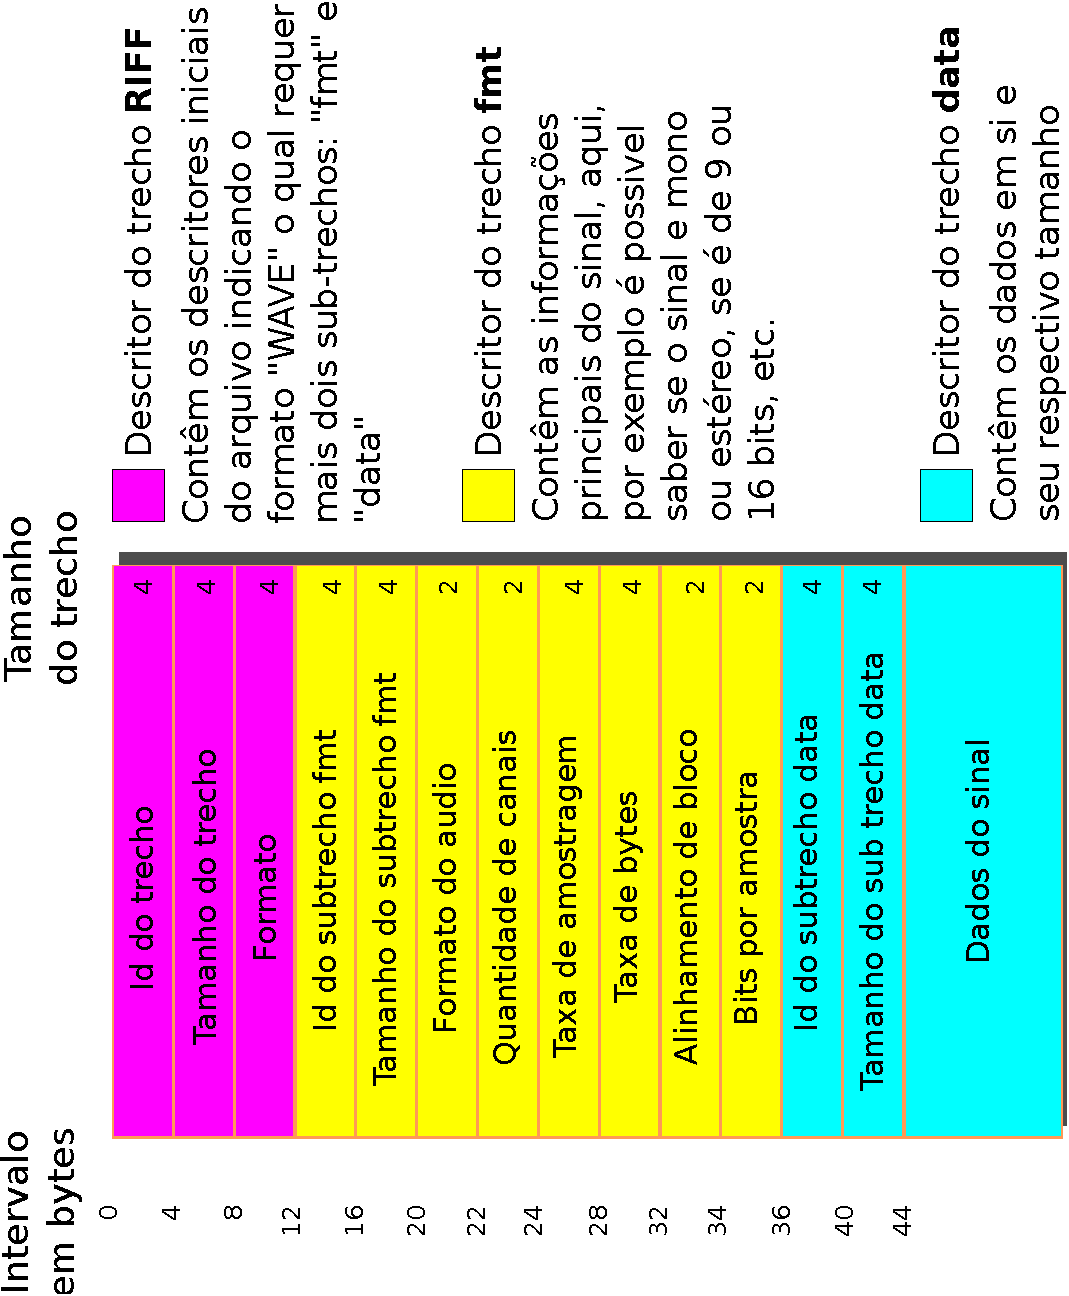
\includegraphics[width=0.70\linewidth, angle=-90]{../monography/images/wavePcmStructure.pdf}
			\label{fig:wavePcmStructure}
		\end{figure}
		\column{0.4\textwidth}
		\begin{itemize}
			\item Formato \textit{wave}.
			\item \textit{Pulse-code modulation} (PCM).
			\item Taxa de amostragem de 44100hz.
			\item Resolução de 16bits
		\end{itemize}
	\end{columns}
\end{frame}
		\begin{frame}
	\frametitle{Sinais Digitais e Sub-amostragem (Downsampling)}
	\begin{itemize}
		\item 
	\end{itemize}
\end{frame}
		\begin{frame}
	\frametitle{Caracterização dos processos de produção da voz humana}
	\only<1>{
		\framesubtitle{Áreas de estudo}
		\begin{itemize}
			\item Fisiológica ou fonética articulatória.
			\item Acústica ou fonética acústica.
			\item Perceptual.
		\end{itemize}
		\textbf{Foco apenas na acústica}
	}
	\only<2>{
		\framesubtitle{Vozeada versus não-vozeada}
		\begin{itemize}
			\item Vozeada: Pregas vocais.
			\item Não vozeada: Sem pregas vocais.
		\end{itemize}
	}
	\only<3>{
		\framesubtitle{Frequência fundamental da voz}
		\begin{itemize}
			\item Conhecida como $F_0$.
			\item Componente periódico resultante da vibração das pregas vocais.
		\end{itemize}
	}
	\only<4>{
		\framesubtitle{Formantes}
		\begin{itemize}
			\item $F_1 \rightarrow$ amplificação  sonora  na  cavidade  oral  posterior,  posição  da  língua  no  plano  vertical.
			\item $F_2 \rightarrow$ cavidade  oral  anterior,  posição  da  língua  no  plano  horizontal.
			\item $F_3 \rightarrow$ cavidades  à  frente  e  atrás  do  ápice  da  língua.
			\item $F_4 \rightarrow$ formato da laringe e da  faringe.
		\end{itemize}
	}
\end{frame}
		\begin{frame}
	\frametitle{Distâncias Euclidiana e Manhattan}
		\par Por definição, as distâncias Euclidiana ($D_E$) e Manhattan ($D_M$) entre dois vetores $x[\cdot]$ e $y[\cdot]$ de tamanho $M$ são dadas, respectivamente, por:
		\begin{equation}
			D_E = \sqrt{\sum\limits_{i=0}^{M-1}(x_i - y_i)^2}  
			\qquad. 
		\end{equation}
		e
		\begin{equation}
			D_M = \sqrt{\sum\limits_{i=0}^{M-1}|x_i - y_i|}   
			\qquad. 
		\end{equation}
\end{frame}


		\begin{frame}
	\frametitle{Escalas de energia}
		\only<1>{
			\framesubtitle{Definições}
			\par As escalas, neste caso, definem os intervalos em que serão calculadas as energias.\newline
			\begin{columns}
				\column{0.5\textwidth}
					\par A energia de um sinal digital $s[\cdot]$ com $M$ amostras é definida como
					\begin{equation}
						E = \sum\limits_{i=0}^{M-1}(s_i)^2 \qquad.   
					\end{equation}
				\column{0.5\textwidth}
					\begin{itemize}
						\item \textbf{Escala BARK:} 20, 100, 200, 300, 400, 510, 630, 770, 920, 1080, 1270, 1480, 1720, 2000, 2320, 2700, 3150, 3700, 4400, 5300, 6400, 7700, 9500, 12000, 15500.
						\item \textbf{Escala MEL:} 20, 160, 394, 670, 1000, 1420, 1900, 2450, 3120, 4000, 5100, 6600, 9000, 14000.
					\end{itemize}
			\end{columns}
		}
		\only<2>{
			\framesubtitle{Cálculo de vetores de características com BARK}
			\begin{figure}
				\centering
				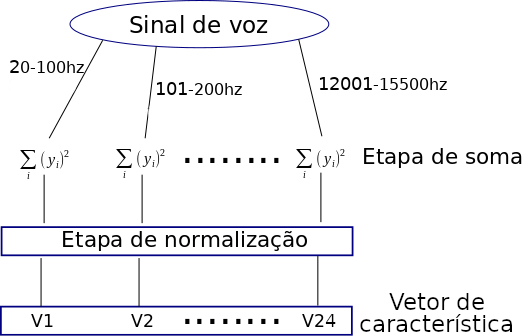
\includegraphics[width=0.7\linewidth]{../monography/images/barkFeatureVect}
			\end{figure}
		}
		\only<3>{
			\framesubtitle{Cálculo de vetores de características com MEL}
			\begin{figure}
				\centering
				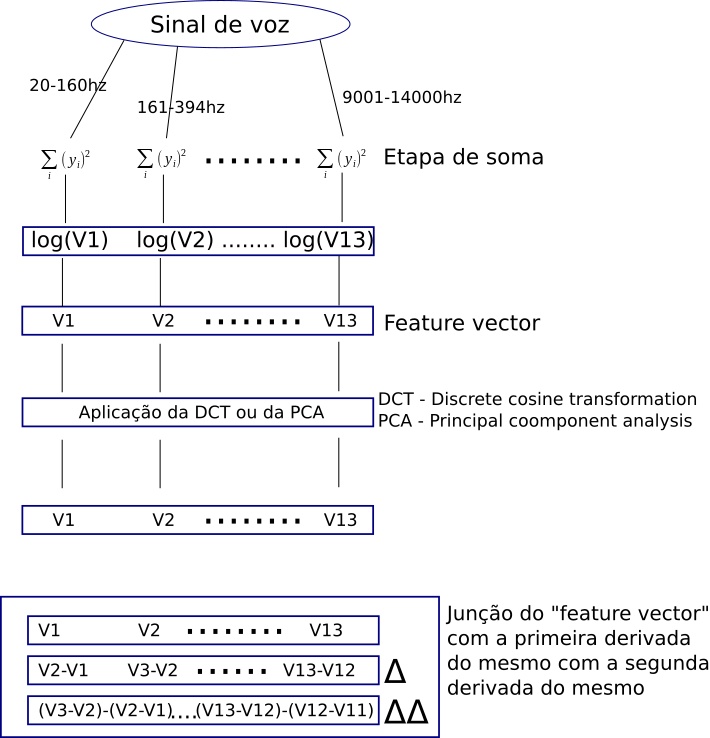
\includegraphics[width=0.5\linewidth]{../monography/images/melFeatureVect}
			\end{figure}
		}
\end{frame}
		\begin{frame}
	\frametitle{Filtros digitais \textit{wavelet}}
	\only<1>{
		\framesubtitle{Propriedades}
		\begin{itemize}
			\item Suporte compacto.
			\item Análise multiresolução.
			\item Wavelet regular e wavelet packet.
			\item Análise detalhada em altas e baixas frequências.
		\end{itemize}
	}
	\only<2>{
		\framesubtitle{Restrição de escopo}
		\begin{itemize}
			\item Domínio discreto.
			\item Apenas transformadas diretas.
			\item Não haverá reconstrução do sinal.
			\item Construção de vetores de características.
		\end{itemize}
	}

	\only<3>{
		\framesubtitle{Resposta em frequência e linearidade}
		\begin{table}[h]
	\centering
	\caption{Algumas das \textit{wavelets} mais usadas e suas propriedades}
	\begin{tabular}{|c|p{75mm}|c|}
			\hline 
			\textbf{Wavelet} & \textbf{Resposta em frequência} & \textbf{Resposta em fase} \\ 
			\hline 
			Haar & Pobre &  Linear \\ 
			\hline 
			Daubechies & mais próxima da ideal à medida que o \newline  suporte aumenta; \textit{maximally-flat}  &  Não linear \\ 
			\hline 
			Symmlets & mais próxima da ideal à medida que o \newline  suporte aumenta; não \textit{maximally-flat}  & Quase linear \\ 
			\hline 
			Coiflets & mais próxima da ideal à medida que o \newline  suporte aumenta; não \textit{maximally-flat}  & Quase linear \\ 
			\hline 
	\end{tabular} 
	\label{tab:waveletsProperties}
	\\Fonte: Elaborado pelo autor, 2021.
\end{table}

	}

	\only<4>{
		\framesubtitle{Algoritmo de Malat}
		\begin{itemize}
			\item \textit{Wavelet} Haar: $h[\cdot] = [\frac{1}{\sqrt{2}}, \frac{1}{\sqrt{2}}]$.
			\item Par ortogonal: $g[\cdot] = [\frac{1}{\sqrt{2}}, \frac{-1}{\sqrt{2}}]$.
			\item sinal: $s[\cdot] = [1,2,3,4]$.
		\end{itemize}
		
		\begin{equation*}
			\begin{pmatrix}
			\frac{1}{\sqrt{2}}, \frac{1}{\sqrt{2}}, 0, 0\\
			\frac{1}{\sqrt{2}}, \frac{-1}{\sqrt{2}}, 0, 0\\
			0, 0, \frac{1}{\sqrt{2}}, \frac{1}{\sqrt{2}}\\
			0, 0, \frac{1}{\sqrt{2}}, \frac{1}{\sqrt{2}}\\
			\end{pmatrix} 
			\cdot
			\begin{pmatrix}
			1\\
			2\\
			3\\
			4\\
			\end{pmatrix} 
			=
			\begin{pmatrix}
			\frac{3}{\sqrt{2}}\\
			\frac{-1}{\sqrt{2}}\\
			\frac{7}{\sqrt{2}}\\
			\frac{-1}{\sqrt{2}}\\
			\end{pmatrix}
			\Rightarrow \Big[
			\frac{3}{\sqrt{2}},
			\frac{7}{\sqrt{2}},
			\frac{-1}{\sqrt{2}},
			\frac{-1}{\sqrt{2}}
			\Big]\qquad.
		\end{equation*}
	}

	\only<5>{
		\framesubtitle{Exemplo de wavelet regular e packet}
		\begin{figure}
			\centering
			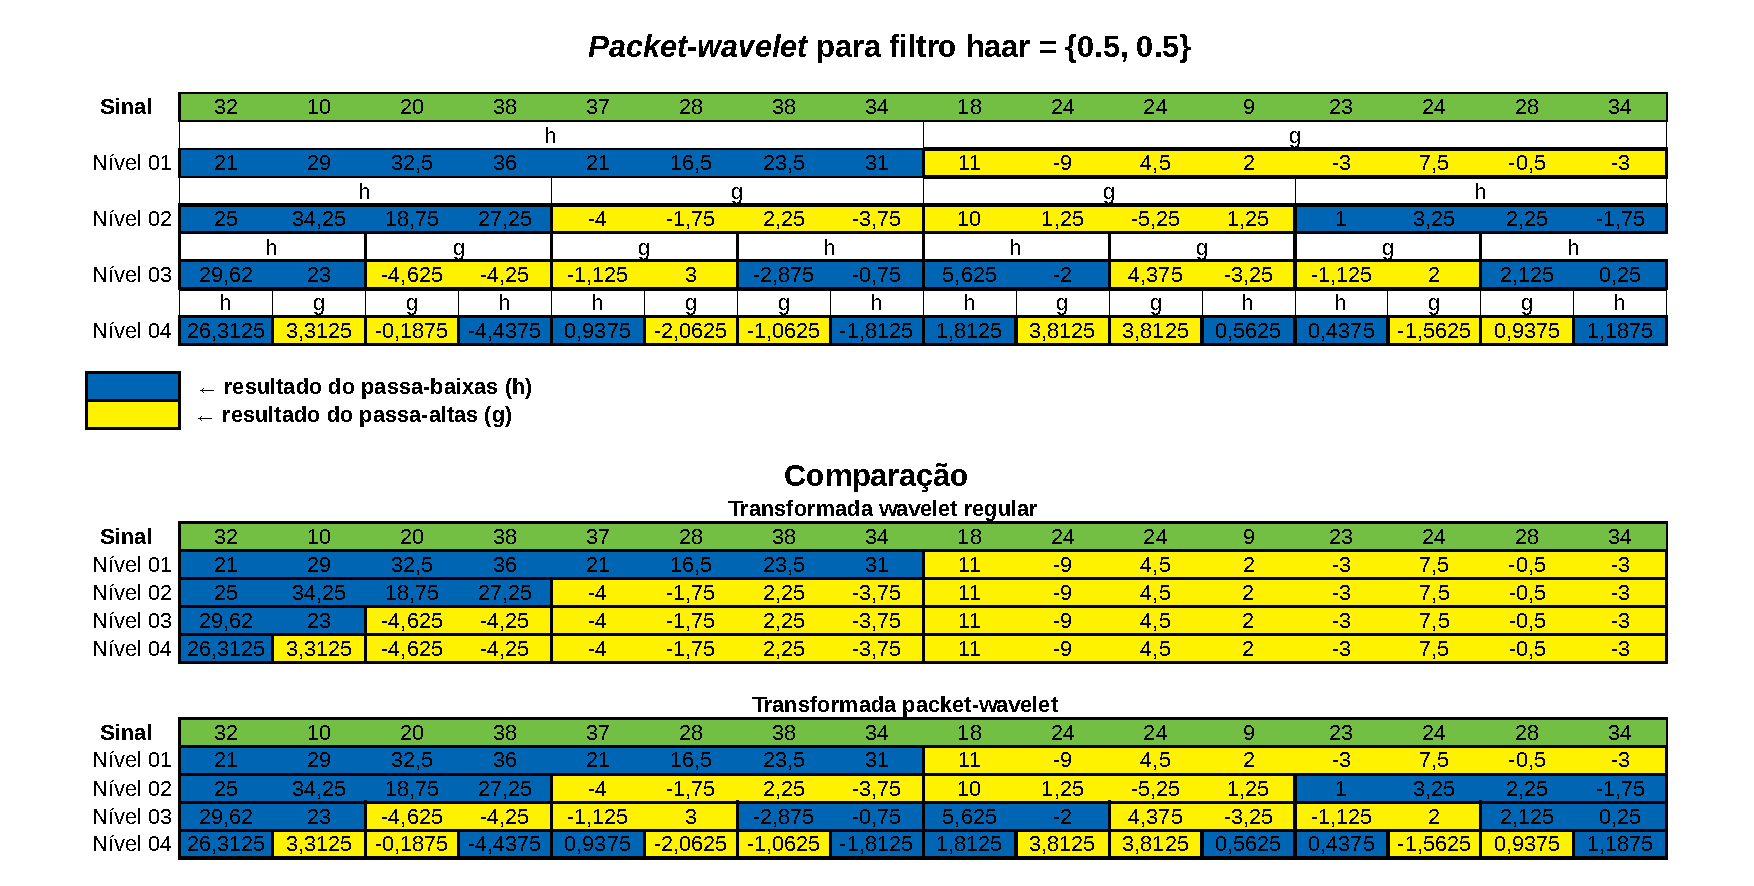
\includegraphics[width=\linewidth]{../monography/images/haarWaveletExamples}
		\end{figure}
	}
\end{frame}








		\begin{frame}
	\frametitle{Engenharia paraconsistente de características}
	\only<1>{
		\framesubtitle{Os vetores de características proporcionam uma boa separação interclasses?}
		\begin{columns}
		\column{.5\textwidth}				
		\begin{figure}
			\centering
			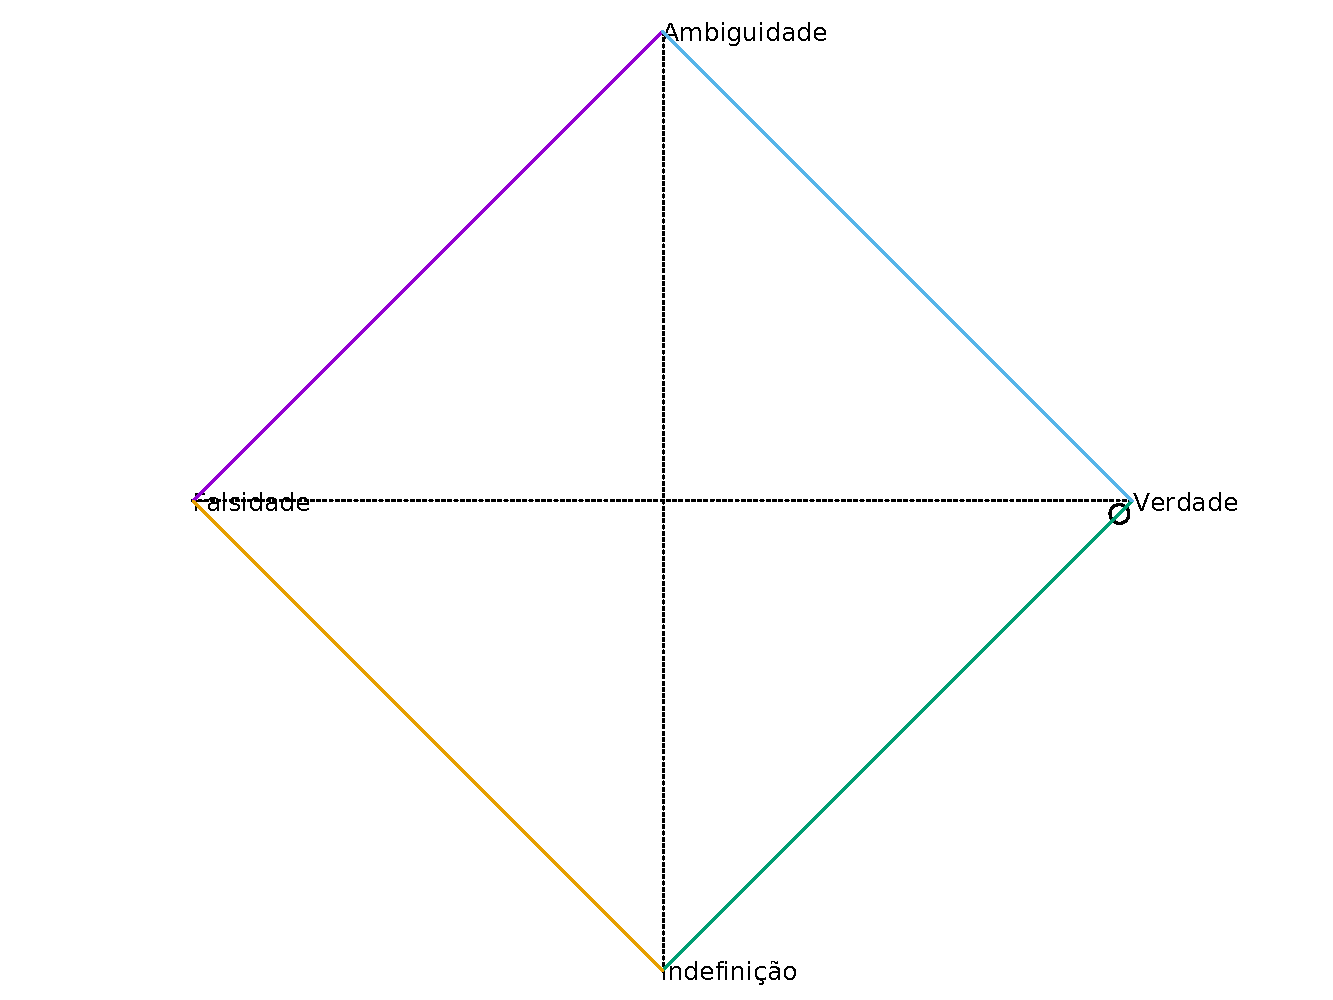
\includegraphics[width=.98\linewidth]{../monography/images/paraconsistentPlane}
			\label{fig:paraconsistentplane}
			\caption{Plano paraconsistente}
		\end{figure}
		\column{.5\textwidth}
		\begin{itemize}
			\item Verdade:\\
		 $\alpha = 1$ e $\beta = 0$.
			\item Ambiguidade:\\
		 $\alpha = 1$ e $\beta = 1$.
			\item Falsidade:\\
		 $\alpha = 0$ e $\beta = 1$.
			\item Indefinição:\\
		 $\alpha = 0$ e $\beta = 0$.
		\end{itemize}
	\end{columns}
	}
	\only<2>{
		\framesubtitle{Cálculo de $\alpha$}
		\begin{columns}
			\column{.5\textwidth}
			\begin{figure}
				\centering
				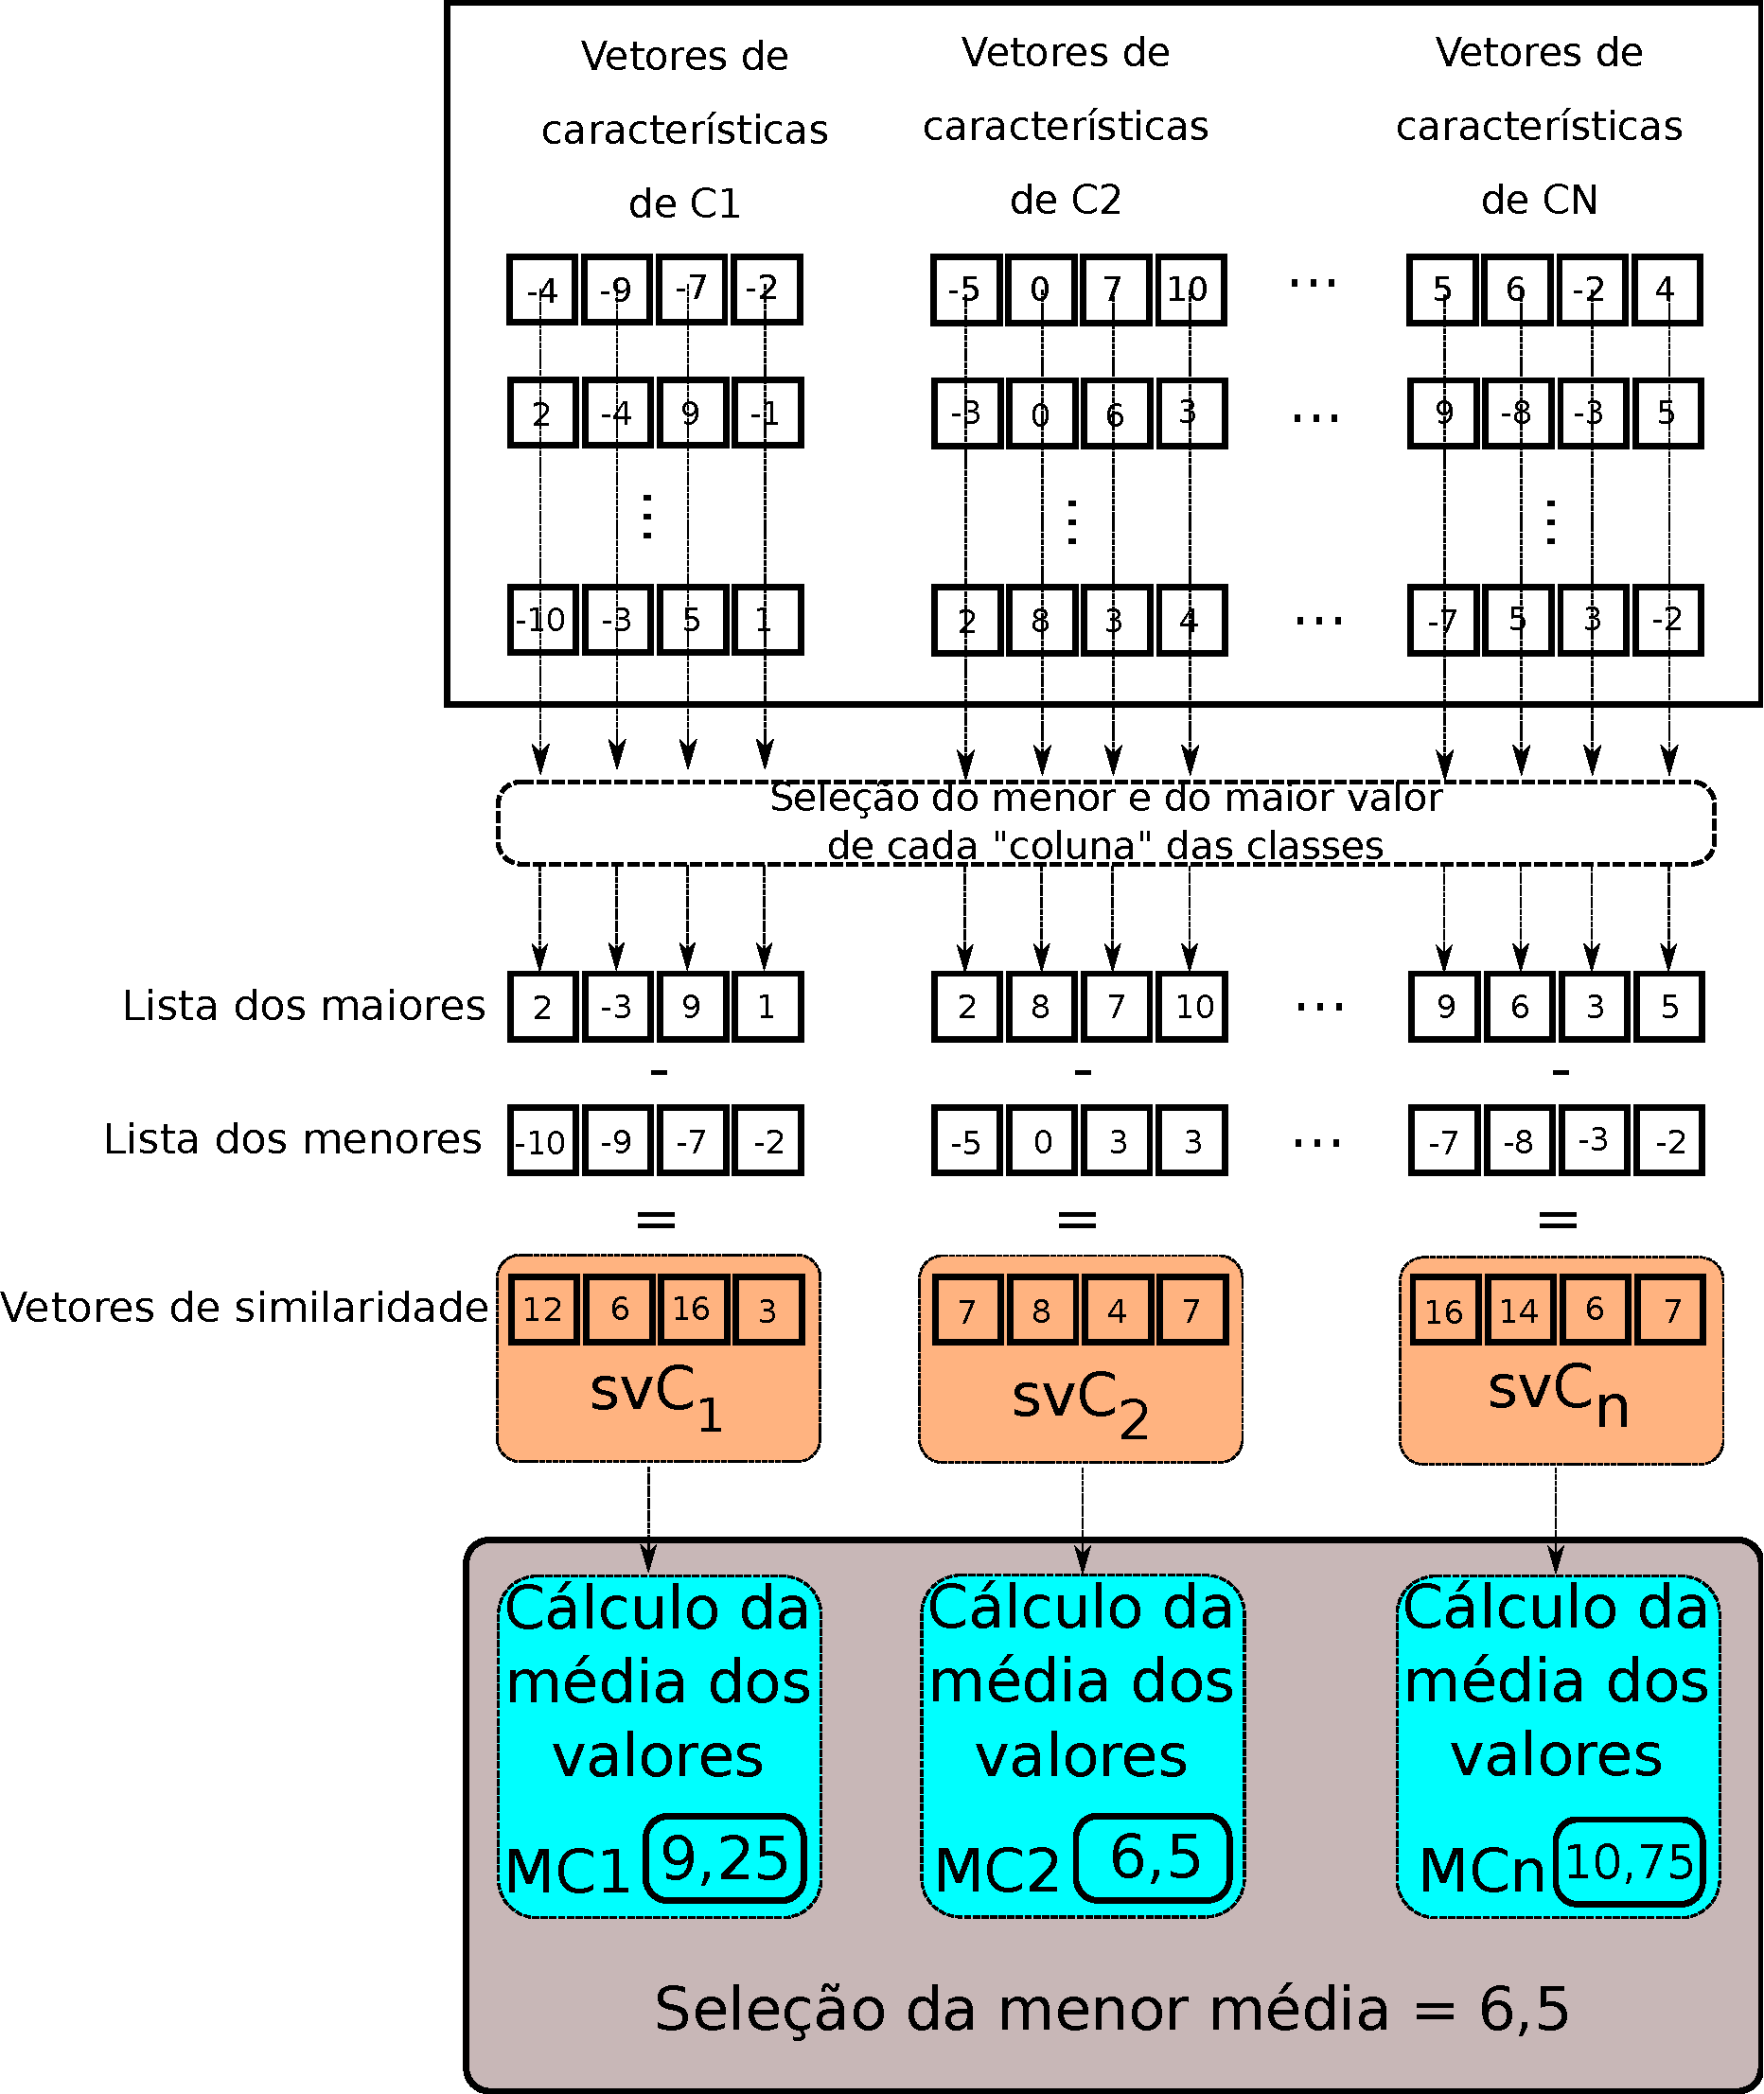
\includegraphics[height=0.82\textheight]{../monography/images/calculoAlpha.pdf}
				\label{fig:calculoalpha}
			\end{figure}
			\column{.5\textwidth}
			\par Menor similaridade intraclasse, $\alpha$
		\end{columns}
	}
	\only<3>{
		\framesubtitle{Cálculo de $\beta$}
		\begin{columns}
			\column{.5\textwidth}
			\begin{figure}
				\centering
				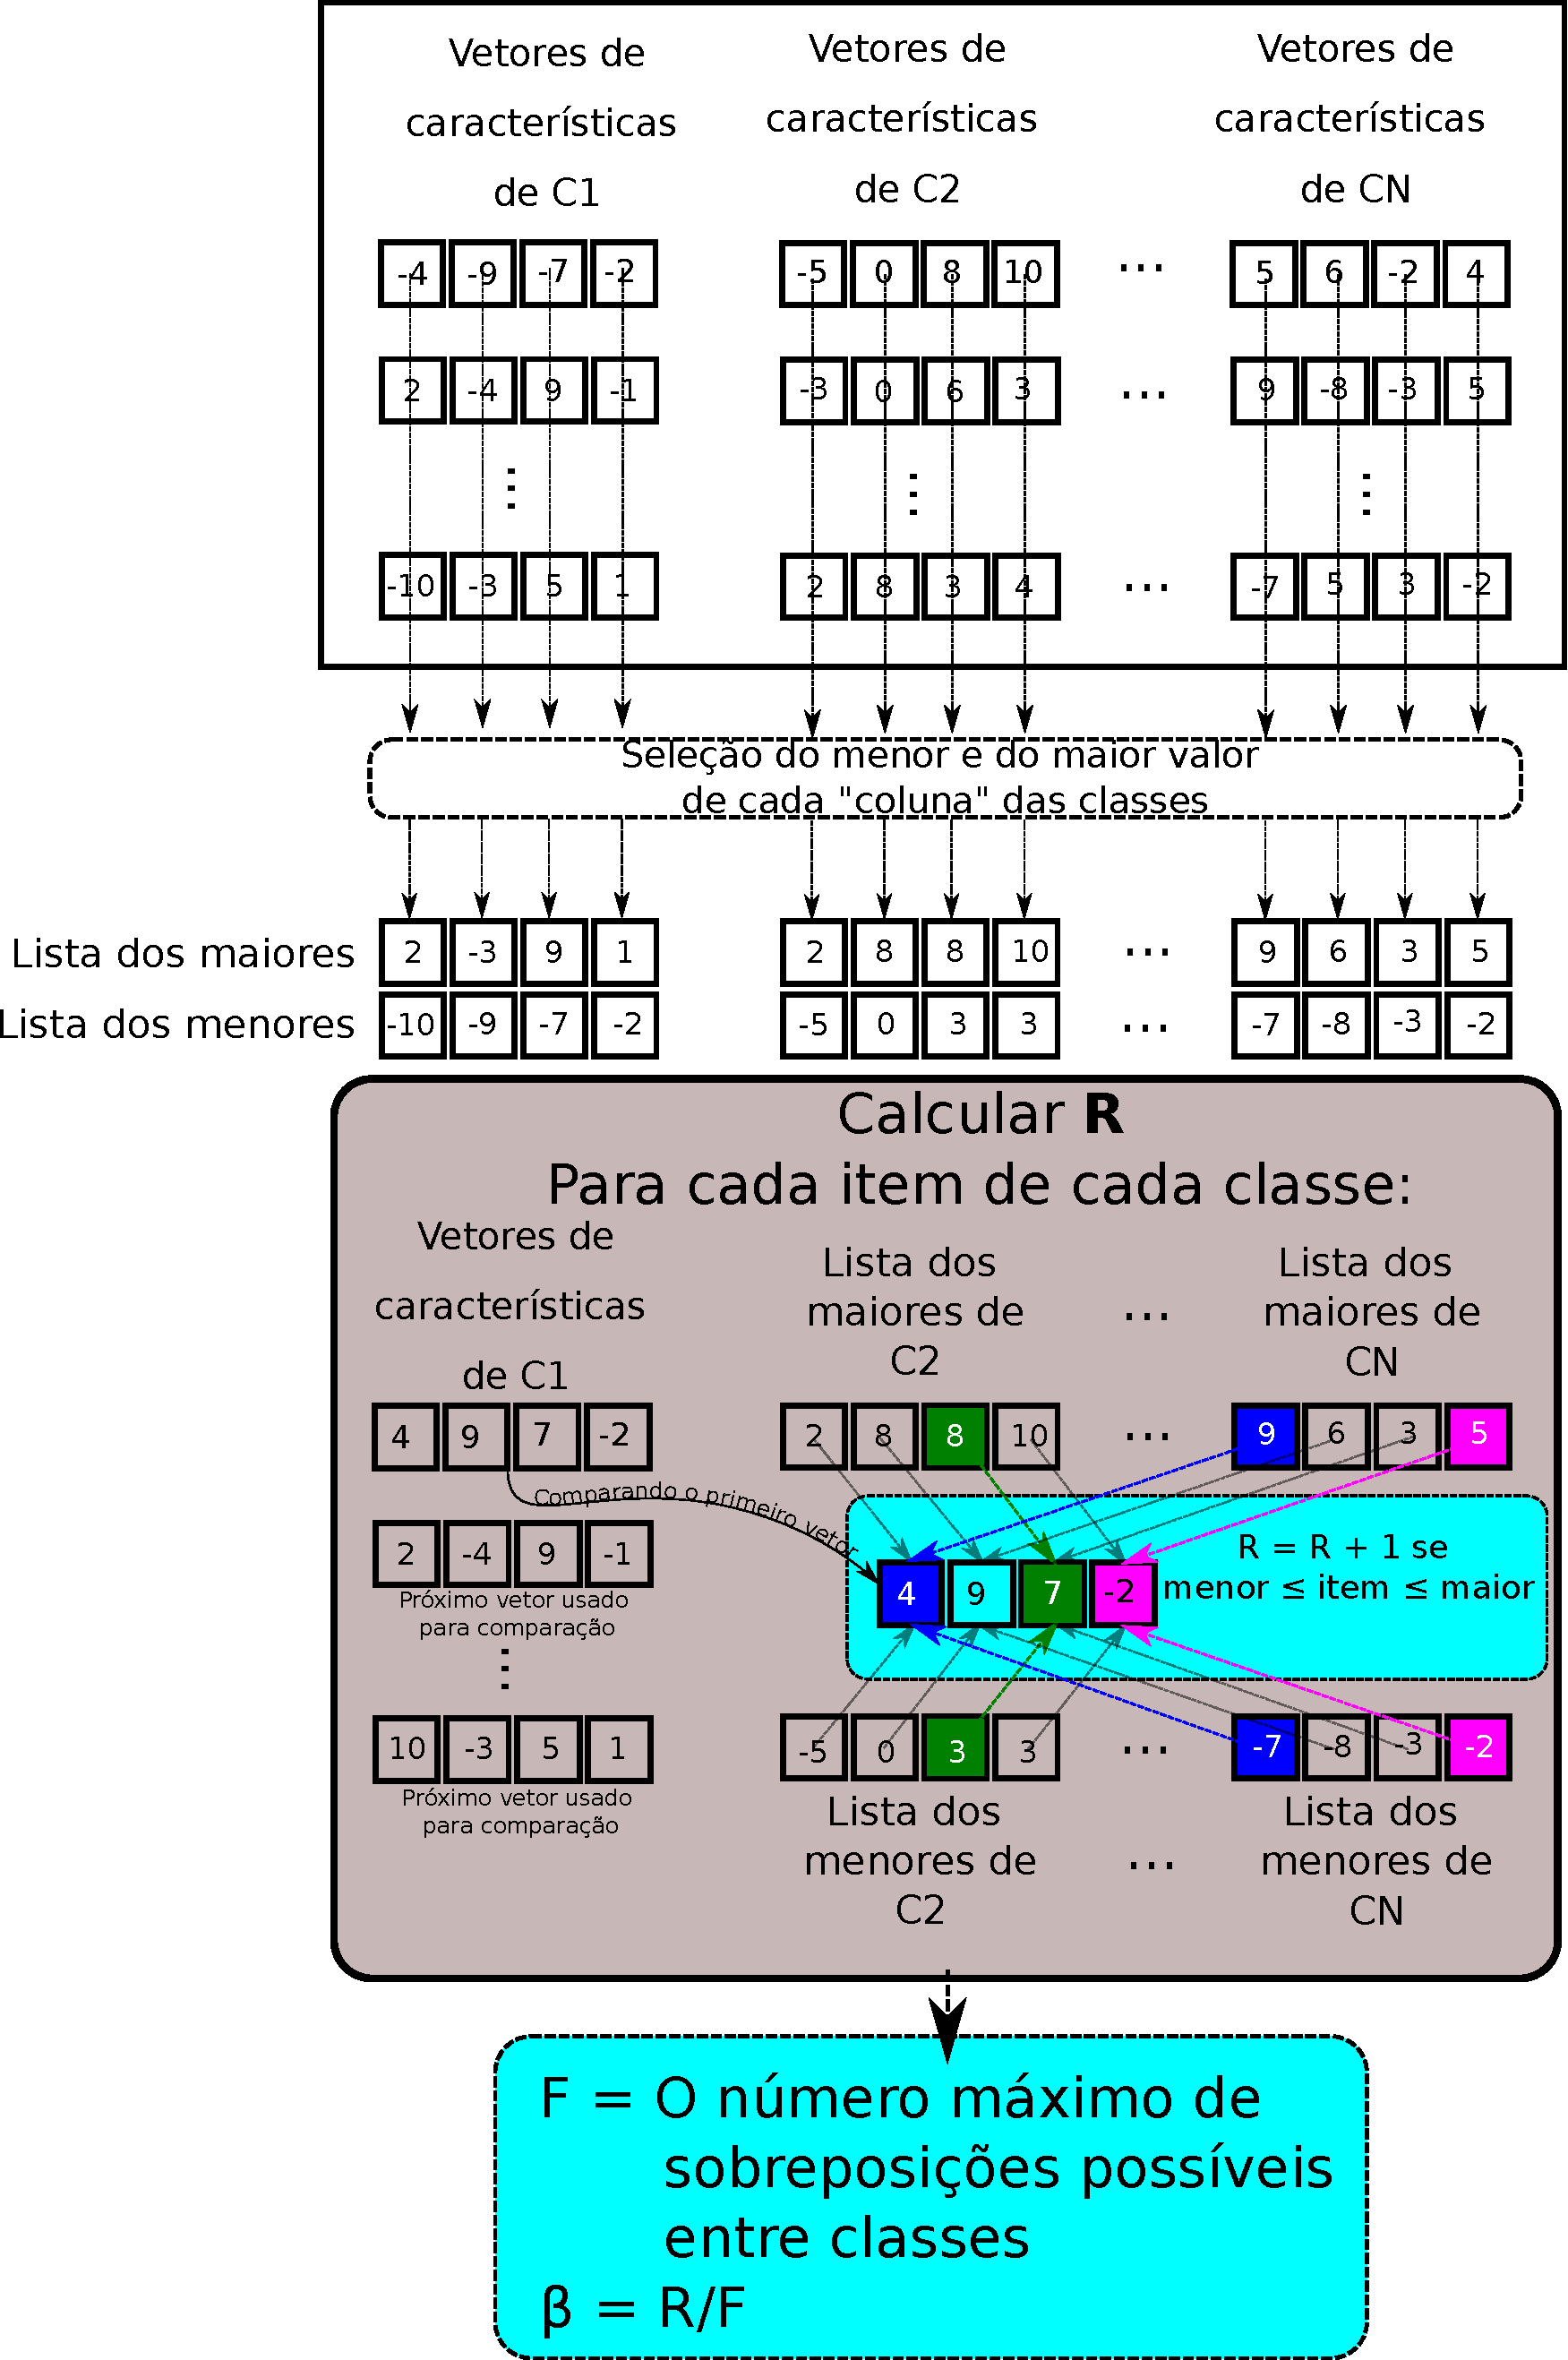
\includegraphics[height=0.82\textheight]{../monography/images/betaCalculation.pdf}
				\label{fig:calculobeta}
			\end{figure}
			\column{.5\textwidth}
			\par Razão de sobreposição interclasse, $\beta$.
		\end{columns}
	}
	\only<4>{
		\framesubtitle{Graus de certeza e contradição}
		\begin{itemize}
			\item Grau de certeza $\rightarrow G_1=\alpha-\beta $.
			\item Grau de contradição $\rightarrow G_2=\alpha+\beta-1 $.				
		\end{itemize}
		Onde: $-1 \leqslant G_1 \leqslant 1$ e  $-1 \leqslant G_2 \leqslant 1\qquad$.\\
		Seja $P=(G_1,G_2)$
		\begin{itemize}
			\item (-1,0) $\rightarrow$ Falsidade;
			\item (1,0) $\rightarrow$ Verdade;
			\item (0,-1) $\rightarrow$ Indefinição;
			\item (0,1) $\rightarrow$ Ambiguidade.
		\end{itemize}
	}
	\only<5>{
		\framesubtitle{Distancias no plano paraconsistente}
		As distâncias$(D)$ do ponto $P=(G_1,G_2)$ dos limites supracitados. Tal cálculo pode ser feito da seguinte forma:
		\begin{equation*}
		D_{-1,0}=\sqrt{(G_1+1)^2+(G_2)^2}\qquad,
		\end{equation*}
		\begin{equation*}
		D_{1,0}=\sqrt{(G_1-1)^2+(G_2)^2}\qquad,
		\end{equation*}
		\begin{equation*}
		D_{0,-1}=\sqrt{(G_1)^2+(G_2+1)^2}\qquad,		
		\end{equation*}
		\begin{equation*}
		D_{0,1}=\sqrt{(G_1)^2+(G_2-1)^2}\qquad,
		\end{equation*}
	}
\end{frame}
	
	\section{Estado-da-arte em Playback Speech Detection}
		\begin{frame}[allowframebreaks]
	\frametitle{Trabalhos}
	\begin{itemize}
		\item \cite{Ren2019}: Energia e outras várias características do espectro do sinal, SVM.
		\item \cite{DiqunYan2019} \textit{Modelo oculto de Markov} (HMM); \textit{Wavelets}, SVM.
		\item \cite{7802552} \textit{Wavelets}, coeficientes cepstrais (SCCs), Modelos de mistura Gaussiana (GMM).
		\item \cite{alluri2019replay} \textit{"Zero time windowing"}(ZTW), análise cepstral do espectro GMM.
		\item \cite{8725688} Coeficientes cepstrais, GMM.
		\item \cite{Hanilci2018} Predição linear, coeficientes cepstrais, GMM.
		\item \cite{ISI:000473343500086} ``Texturas de voz'', padrões binários locais (LBP) e seus respectivos histogramas, SVM.
		\item Uma abordagem que combina análise de sinal de fala usando a \textit{Transformada Constante Q} (CQT) com o processamento cepstral foi mostrada no artigo \cite{TODISCO2017516}.
		\item No artigo \cite{Patel2015} é usada a \textit{Transformação Auditiva (TU)} que tem como base a transformada \textit{wavelet}, e a \textit{Cochlear Filter Cepstral Coefficients (CFCC)} juntamente com  \textit{estimação da frequência instantânea (IF)}.
		\item \cite{ISI:000490497200068} Partes não vozeadas da fala, três GMMs.
		\item \cite{ISI:000465363900136} amplitude instantânea vinda de flutuações de energia, GMM.
		\item \cite{ISI:000465363900139} Diferenças entre bandas de frequências específicas, \textit{predição linear em domínio de frequência}(FDLP), GMMs.
		\item \cite{Suthokumar2018} \textit{Modulation  spectral  centroid  frequency}, \textit{long term spectral average}, GMM.
		\item \cite{ISI:000458728700054} Envelopamento das amplitudes e das frequências instantâneas em cada banda estreita filtrada, GMM.
		\item \cite{ISI:000392503100008} \textit{Gammatone frequency cepstral coefficients}(MGFCC), GMM.
		\item \cite{8396208} \textit{Hashing} sensível a locus(LSH), MFCC e LSH, tabela \textit{hash}. 
	\end{itemize}
\end{frame}
\begin{frame}
	\frametitle{Comparativo}
		\begin{columns}
			\column{0.5\textwidth}
				\par \textbf{Referências}
				\begin{itemize}
					\item Apenas escala MEL.
					\item Classificadores simples.
					\item Uso escasso de wavelets.
					\item Uso do EER como métrica.
					\item Sem metodologia de comparação automática.
				\end{itemize}
			\column{0.5\textwidth}
				\par \textbf{Dissertação}
				\begin{itemize}
					\item Escalas MEL e BARK.
					\item Classificadores simples.
					\item Uso intensivo wavelets.
					\item Uso de EER e acurácia como métrica.
					\item Comparação automática baseada na engenharia paraconsistente de características.
				\end{itemize}
		\end{columns}
\end{frame}
		
	\section{Contextualização}
		\begin{frame}
	\frametitle{Contextualização}
	\begin{itemize}
		\item Características mais disjuntas possíveis para de ``locutor autêntico'' e ``ataque de \textit{voice spoofing}''.
		\item \textit{Wavelet}: Boa resolução em relação às dimensões de tempo e frequência.
		\item Análise paraconsistente de acordo com o trabalho \cite{8588433}.
	\end{itemize}
\end{frame}

	\section{Abordagem proposta}
		\begin{frame}
	\frametitle{A Base de Sinais de Voz}
	\only<1>{
		\framesubtitle{Coleta dos dados}
		\begin{itemize}
			\item 20 pessoas.
			\item Ambos sexos.
			\item Idades entre 7 e 67 anos.
			\item Dígitos falados de 0 a 9.
			\item Língua portuguesa e inglesa.
			\item Total de 820 sinais entre genuínos e falsificados.
			\item Quantização de 16 bits.
			\item Taxa de amostragem 44100Hz.
		\end{itemize}
	}
	\only<2>{
		\framesubtitle{Organização dos dados}
		\begin{textblock*}{\linewidth}(0cm,0.4cm)
			\begin{figure}[t]
				\centering
				\subfloat[0.33\textwidth][Base em nível 1]{
					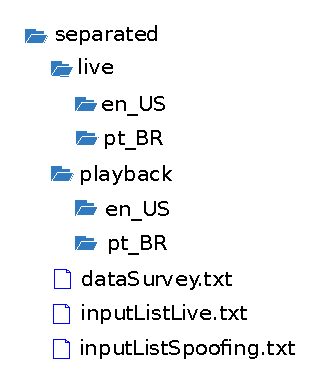
\includegraphics{../monography/images/directoryStructLevel01.pdf}
					\label{fig:directorystructlevel01}
				}
				\subfloat[0.33\textwidth][Base em nível 2]{
					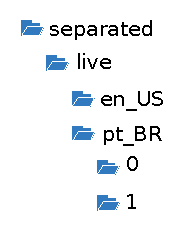
\includegraphics{../monography/images/directoryStructLevel02.pdf}
					\label{fig:directorystructlevel02}
				}
				\subfloat[0.33\textwidth][Base em nível 3]{
					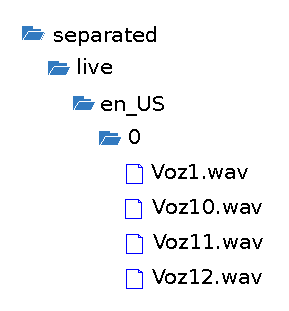
\includegraphics{../monography/images/directoryStructLevel03.pdf}
					\label{fig:directorystructlevel03}
				}
				\caption{Organização da base de dados}
				\label{fig:directorystructlevel010203}
			\end{figure}
		\end{textblock*}
	}
\end{frame}
		\begin{frame}
	\frametitle{Estrutura da Estratégia Proposta}
		\only<1>{
			\framesubtitle{Diagrama}
			\begin{textblock*}{\linewidth}(0.3cm,2cm)
				\begin{figure}[h]
	\centering
	\caption{Estrutura da estratégia proposta}
	\scalebox{0.75}	{
		\begin{tikzpicture} 
			\node (z1)[shape=rectangle, rounded corners, draw, align=center, top color=white, bottom color=red!50] 
			at (0,2){
				\textbf{Sinal de} \\ \textbf{entrada} \\ \textbf{sob} \\ \textbf{análise}
			}; 
				
			\node (z2)[shape=rectangle, rounded corners, draw, align=center, top color=white, bottom color=yellow!50] 
			at (5.5,2){
				pré-processamento \\ e extração de \\ características no \\ domínio \textit{wavelet}
			}; 	
			
			\node (z3)[shape=rectangle, rounded corners, draw, align=center, top color=white, bottom color=yellow!50] 
			at (11,2){
				agrupamento energético \\ nas bandas Bark / Mel
			}; 	
			
			\node (z4)[shape=rectangle, rounded corners, draw, align=center, top color=white, bottom color=yellow!50] 
			at (16.5,2){
				análise paraconsistente \\ de características
			}; 
			
			\node (z5)[shape=rectangle, rounded corners, draw, align=center, top color=white, bottom color=yellow!50] 
			at (16.5,0.25){
				seleção da melhor combinação \\ agrupamento energético + wavelet
			}; 
					
			\node (z6)[shape=circle, draw, align=center, top color=white, bottom color=blue!10] 
			at (7,0.25) {};
			
			\node (z7)[shape=rectangle, rounded corners, draw, align=center, top color=white, bottom color=yellow!50] 
			at (7,-1.25) {
				classificador \\ por distâncias \\ ou SVM
			};
			
			\node (z8)[shape=rectangle, rounded corners, draw, align=center, top color=white, bottom color=green!80] 
			at (12,-1.25) {
				\textbf{Resultados}
			};
			
			\path[->] (z1) edge (z2);
			\path[->] (z2) edge (z3);
			\path[->] (z3) edge (z4);
			\path[->] (z4) edge (z5);
			\path[->] (z5) edge (z6);
			\path[->] (z6) edge (z7);	
			\path[->] (z7) edge (z8);
		\end{tikzpicture}
	}
	\label{fig_arq}
	\\Fonte: Elaborado pelo autor, 2021.
\end{figure}
			\end{textblock*}
		}
		\only<2>{
			\framesubtitle{Wavelets usadas}
				\begin{itemize}
					\item Haar.
					\item Beylkin com suporte 18.
					\item Vaidyanathan de suporte 24.
					\item Daubechies de	suportes 4 até 76.
					\item Symmlets com suportes 8, 16 e 32.
					\item Coiflets com suportes 6, 12, 18, 24 e 30.
				\end{itemize}
		}
		\only<3>{
			\framesubtitle{Métricas}
				\begin{itemize}
					\item Tabela de confusão.
					\begin{itemize}
						\item EER (Equal Error Rate).
						\item Acurácia e seu respectivo desvio padrão.
					\end{itemize}
				\end{itemize}
		}
		\only<4>{
			\framesubtitle{Tabela de confusão}
				\begin{itemize}
					\item \textbf{TP}: Quantidade de itens verdadeiros classificados como tal (\textit{True Positive}).
					\item \textbf{TN}: Quantidade de itens falsos classificados como tal (\textit{True Negative}).
					\item \textbf{FN}: Quantidade de itens verdadeiros classificados como falsos (\textit{False Negative}).
					\item \textbf{FP}: Quantidade de itens falsos classificados como verdadeiros (\textit{False Positive}).
				\end{itemize} 
				\begin{table}
\newcommand{\mc}[3]{\multicolumn{#1}{#2}{#3}}
\definecolor{tcB}{rgb}{0.447059,0.74902,0.266667}
\definecolor{tcC}{rgb}{0,0,0}
\definecolor{tcD}{rgb}{0,0.4,0.701961}
\definecolor{tcA}{rgb}{0.65098,0.65098,0.65098}
\begin{center}
	\begin{tabular}{ccc}
		% use packages: color,colortbl
		\mc{1}{l}{} & \mc{1}{>{\columncolor{tcA}}c}{\textbf{Verdadeiro}} & \mc{1}{>{\columncolor{tcA}}c}{\textbf{Falso}}\\

		\mc{1}{>{\columncolor{tcA}}r}{\textbf{Verdadeiro}} & \mc{1}{>{\columncolor{tcB}}c}{\textcolor{tcC}{VV}} & \mc{1}{>{\columncolor{tcD}}c}{\textcolor{tcC}{FV}}\\

		\mc{1}{>{\columncolor{tcA}}r}{\textbf{Falso}} & \mc{1}{>{\columncolor{tcD}}c}{\textcolor{tcC}{FF}} & \mc{1}{>{\columncolor{tcB}}c}{\textcolor{tcC}{VF}}
	\end{tabular}
	\caption{Exemplo de matriz de confusão}
	\label{tab:confusionMatrixSample}
\end{center}
\end{table}

		}
		\only<5>{
			\framesubtitle{Acurácia e EER}
				\begin{columns}
					\column{.5\textwidth}
					\begin{equation}
						acuracia = \dfrac{TP + TN}{N} \qquad.
						\label{eq:calculoDaAcuracia}
					\end{equation}
					
					\column{.5\textwidth}
					\par São calculadas tabelas de confusão por um número suficiente de vezes até que \textbf{\textit{FAR} = \textit{FRR} = \textit{EER}}, a cada ciclo os vetores de características são comutados de forma aleatória.\newline

					\begin{equation}
						FAR=\dfrac{FP}{TN+FP} \qquad.
						\label{eq:FAR}
					\end{equation}
					
					\begin{equation}
						FRR=\dfrac{FN}{TP+FN} \qquad.
						\label{eq:FRR}
					\end{equation}
				\end{columns}
		}
\end{frame}
		\begin{frame}
	\frametitle{Procedimento 01}
		\only<1>{
			\framesubtitle{Características}
				\begin{itemize}
					\item MEL: 13 coeficientes.
					\item BARK: 24 coeficientes.
					\item Redimensionar o sinal.
					\item Determinar o máximo de transformações.
					\item Transformadas wavelet-packet até o nível máximo.
					\item Selecionar a melhor combinação \textit{wavelet}/escala.
				\end{itemize}
		}
		\only<2>{
			\framesubtitle{Comprimento e máximo de transformações do sinal}
			\par Determinação do tamanho ótimo para as transformações
			\begin{equation}
				tamanhoOtimo=2^{proxInt(\log_{2}tamanho)}
				\label{eq:optimalSize}
			\end{equation} 
			
			\par Quantidade máxima de transformações
			\begin{equation}
				maxTrans=\log_{2}(tamanho) \qquad.
				\label{eq:maxWaveletTransf}
			\end{equation}
		}
		\only<3>{
			\framesubtitle{Algoritmo}
			\begin{lstlisting}[language=C++]
// Carregue para a memoria um dos conjuntos de amostra
for (listaDeAmostras : {listaComVoiceSpoofing, listaSemVoiceSpoofing}) {
	// Selecione o proximo tipo de wavelet
	for (wavelet : wavelets) {
		// Selecione entre BARK ou MEL
		for (barkOuMel : {BARK, MEL}) {
			// Selecione o proximo sinal dentro da amostra
			for (sinal : listaDeAmostras) {
				tamanhoOtimo=calcularTamanhoOtimo(sinal);
				redimensionar(sinal, tamanhoOtimo);
				sinalTransformado=wavelet(sinal, wavelet);
				energias=calcularEnergias(sinalTransformado, barkOuMel);
				energias=normalizar(energias);
				
				// Armazene os resultados
				resultados[wavelet.nome()][barkOuMel][listaDeAmostras.nome()].adicionar(energias);
			}
		}
	}
}
// Posicione os resultados no plano paraconsistente
mostraResultadosNoPlanoParaconsistente(resultados);
\end{lstlisting}
		}
\end{frame}

\begin{frame}
	\frametitle{Procedimento 02}
	\only<1>{
		\framesubtitle{Características}
		\begin{itemize}
			\item Bandas críticas: BARK.
			\item Wavelet: Haar.
			\item Modelos de 10\% 20\% 30\% 40\% e 50\%.
			\item Sorteio aleatório de vetores de características.
			\item Verifica a acurácia e o EER de classificadores \textit{pattern-matching} por distâncias Euclidiana e Manhattan.
		\end{itemize}
	}
	\only<2>{
		\framesubtitle{Algoritmo}
		\begin{lstlisting}[language=C++, caption={Procedure 02 algorithm}, label={lst:experiment02Algo}]
modelProportion={0.1, 0,2, 0,4, 0,5};
genuineModel = spoofingModel= genuineTest = spoofingTest = accuracyList = {};
for (distance : {Euclidian, Manhattan}) {
	for(percentage : modelProportion){
		for(testCounter = 0; testCounter < 300; testCounter++){
			// Choose feature vectors randomly from spoofing set
			// to build the model according to the proportions chosen.
			chooseRamdomly(voiceSpoofingSet, percentage, spoofingModel, spoofingTest);
			// Choose feature vectors randomly from genuine set
			// to build the tests according to the proportion chosen
			chooseRamdomly(genuineSet, percentage, genuineModel, genuineTest);
			
			trainClassificator("spoofing", spoofingModel);
			trainClassificator("genuine", genuineModel);
			// Classify the spoofing tests against the 
			// spoofing model and fill the confusion tables
			for(signal : spoofingTest){
				fillConfusionTable(signal, "spoofing");
			} 
			// Classify the genuine tests against the
			// genuine model and fill the confusion tables
			for(signal : genuineTest){
				fillConfusionTable(signal, "genuine");
			}

			accuracy=calculateAccuracy();
			
			// Store the accuracies for each percentage
			accuracyList[percentage].add(accuracy);

			// Store the best accuracy and its respective confusion table
			if(isTheBestAccuracy(accuracy)){
				saveAccuracyAndItsConfusionTable();
			}
			
			// Store the worst accuracy and its respective confusion table
			if(isTheWorstAccuracy(accuracy)){
				saveAccuracyAndItsConfusionTable();
			}
		}
		
		// Calculate and save the standard deviation for current proportion
		calculateAndSaveTheStandardDeviation(accuracyList[percentage]);
	}
}				
\end{lstlisting}
	}
\end{frame}

\begin{frame}
	\frametitle{Procedimento 03}
	\only<1>{
		\framesubtitle{Características}
		\begin{itemize}
			\item Bandas críticas: BARK.
			\item Wavelet: Haar.
			\item Modelos de 10\% 20\% 30\% 40\% e 50\%.
			\item Sorteio aleatório de vetores de características.
			\item Verifica a acurácia e o EER de uma \textit{Support Vector Machine (SVM)}.
		\end{itemize}
	}
	\only<2>{
		\framesubtitle{Características da SVM}
		\begin{figure}
	\centering
	\scalebox{2}{
				\begin{tikzpicture}
	%input layer
	\node (input1) at (0.65,2.0) {};
	\draw[->,in=180,out=0] (1.0,2.0) to (1.35,2.0);
	\node (input2) at (0.65,1.5) {};
	\draw[->,in=180,out=0] (1.0,1.5) to (1.35,1.5);
	\node (input3) at (0.65,1.0) {};
	\draw[->,in=180,out=0] (1.0,1.0) to (1.35,1.0);
	\node (input3) at (0.65,0.0) {};
	\draw[->,in=180,out=0] (1.0,0.0) to (1.35,0.0);
	\node (IL_N1) at (1.5,2.0) {}; \filldraw[fill=gray!30] (1.5,2.0) circle (0.15cm);
	\node (IL_N2) at (1.5,1.5) {}; \filldraw[fill=gray!30] (1.5,1.5) circle (0.15cm);
	\node (IL_N3) at (1.5,1.0) {}; \filldraw[fill=gray!30] (1.5,1.0) circle (0.15cm);
	\node at (1.5,0.625) {$\vdots$};
	\node (IL_Nn) at (1.5,0.0) {}; \filldraw[fill=gray!30] (1.5,0.0) circle (0.15cm);
	
	%hidden layer 
	\node (HL_N1) at (3.5,2.5) {}; \filldraw[fill=blue!20] (3.55,2.5) circle (0.15cm);
	\node (HL_N2) at (3.5,2.0) {}; \filldraw[fill=blue!20] (3.55,2.0) circle (0.15cm);
	\node (HL_N3) at (3.5,1.5) {}; \filldraw[fill=blue!20] (3.55,1.5) circle (0.15cm);
	\node (HL_N4) at (3.5,1.0) {}; \filldraw[fill=blue!20] (3.55,1.0) circle (0.15cm);
	\node at (3.55,0.625) {$\vdots$};
	\node (HL_Nn-1) at (3.5,0.0) {}; \filldraw[fill=blue!20] (3.55,0.0) circle (0.15cm);	
	\node (HL_Nn) at (3.5,-0.5) {}; \filldraw[fill=blue!20] (3.55,-0.5) circle (0.15cm);	
	\draw[->,in=180,out=0] (IL_N1)+(1.5mm,0) to (HL_N1);
	\draw[->,in=180,out=0] (IL_N1)+(1.5mm,0) to (HL_N2);
	\draw[->,in=180,out=0] (IL_N1)+(1.5mm,0) to (HL_N3);
	\draw[->,in=180,out=0] (IL_N1)+(1.5mm,0) to (HL_N4);
	\draw[->,in=180,out=0] (IL_N1)+(1.5mm,0) to (HL_Nn-1);
	\draw[->,in=180,out=0] (IL_N1)+(1.5mm,0) to (HL_Nn);
	
	\draw[->,in=180,out=0] (IL_N2)+(1.5mm,0) to (HL_N1);
	\draw[->,in=180,out=0] (IL_N2)+(1.5mm,0) to (HL_N2);
	\draw[->,in=180,out=0] (IL_N2)+(1.5mm,0) to (HL_N3);
	\draw[->,in=180,out=0] (IL_N2)+(1.5mm,0) to (HL_N4);
	\draw[->,in=180,out=0] (IL_N2)+(1.5mm,0) to (HL_Nn-1);
	\draw[->,in=180,out=0] (IL_N2)+(1.5mm,0) to (HL_Nn);
	
	\draw[->,in=180,out=0] (IL_N3)+(1.5mm,0) to (HL_N1);
	\draw[->,in=180,out=0] (IL_N3)+(1.5mm,0) to (HL_N2);
	\draw[->,in=180,out=0] (IL_N3)+(1.5mm,0) to (HL_N3);
	\draw[->,in=180,out=0] (IL_N3)+(1.5mm,0) to (HL_N4);
	\draw[->,in=180,out=0] (IL_N3)+(1.5mm,0) to (HL_Nn-1);
	\draw[->,in=180,out=0] (IL_N3)+(1.5mm,0) to (HL_Nn);
	
	\draw[->,in=180,out=0] (IL_Nn)+(1.5mm,0) to (HL_N1);
	\draw[->,in=180,out=0] (IL_Nn)+(1.5mm,0) to (HL_N2);
	\draw[->,in=180,out=0] (IL_Nn)+(1.5mm,0) to (HL_N3);
	\draw[->,in=180,out=0] (IL_Nn)+(1.5mm,0) to (HL_N4);
	\draw[->,in=180,out=0] (IL_Nn)+(1.5mm,0) to (HL_Nn-1);
	\draw[->,in=180,out=0] (IL_Nn)+(1.5mm,0) to (HL_Nn);
	
	%output layer
	\node (OL_N1) at (5.5,1.0) {}; \filldraw[fill=red!40] (5.55,1.0) circle (0.15cm);
	
	\draw[->,in=180,out=0] (HL_N1)+(2mm,0) to (OL_N1);
	\draw[->,in=180,out=0] (HL_N2)+(2mm,0) to (OL_N1);
	\draw[->,in=180,out=0] (HL_N3)+(2mm,0) to (OL_N1);
	\draw[->,in=180,out=0] (HL_N4)+(2mm,0) to (OL_N1);
	\draw[->,in=180,out=0] (HL_Nn-1)+(2mm,0) to (OL_N1);
	\draw[->,in=180,out=0] (HL_Nn)+(2mm,0) to (OL_N1);
	%
	\draw[snake=brace,mirror snake,raise snake=45pt,brown] (1.25,1.25) -- (1.75,1.25) node[black,midway,yshift=-50pt,below]{\tiny camada de} node[black,midway,yshift=-58pt,below]{\tiny entrada com} node[black,midway,yshift=-66pt,below]{\tiny $R$ elementos}
	node[black,midway,yshift=-74pt,below]{\tiny passivos};
	\draw[snake=brace,mirror snake,raise snake=45pt,brown] (3.25,0.75) -- (3.75,0.75) node[black,midway,yshift=-50pt,below]{\tiny camada} node[black,midway,yshift=-58pt,below]{\tiny intermediária} node[black,midway,yshift=-66pt,below]{\tiny com $X$ neurônios}
	node[black,midway,yshift=-74pt,below]{\tiny ativos não-lineares};
	\draw[snake=brace,mirror snake,raise snake=45pt,brown] (5.25,1.75) -- (5.75,1.75) node[black,midway,yshift=-50pt,below]{\tiny camada de} node[black,midway,yshift=-58pt,below]{\tiny saída com} node[black,midway,yshift=-66pt,below]{\tiny um elemento}
	node[black,midway,yshift=-74pt,below]{\tiny ativo linear};
	%
	\node (OUT) at (6.5,1.0) {\tiny resultado}; 
	\draw[->,in=180,out=0] (OL_N1)+(2mm,0) to (OUT);	
	
	\node at (4,2.6) {\tiny $p_0$}; 
	\node at (4,2.1) {\tiny $p_1$}; 
	\node at (4,1.65) {\tiny $p_2$}; 
	\node at (4,1.2) {\tiny $p_3$}; 
	\node at (4,0.2) {\tiny $p_{X-2}$}; 
	\node at (4,-0.3) {\tiny $p_{X-1}$}; 
\end{tikzpicture}
	}
	\caption{Estrutura da SVM para o procedimento 03 com $R$ neurônios na camada de entrada, sendo $R$ a dimensão dos vetores de características, e $X$ neurônios na camada intermediária, sendo $X$ o número de casos de treinamento}
	\label{fig:3layersSVM}
\end{figure} 
	}
	\only<3>{
		\framesubtitle{Características da SVM}
		\begin{itemize}
			\item Três camadas: Entrada, segunda com elementos ativos não-lineares de núcleos Gaussianos e saída; 
			\item Inexistem pesos entre a camada de entrada e a camada intermediária;
			\item A saída de cada elemento da camada intermediária conecta-se com o único elemento da camada de saída por meio dos pesos $p_0, p_1, .... p_{X-1}$;
			\item O valor de saída consiste na combinação linear dos pesos com os valores recebidos como entrada da camada de saída;
			\item Solução direta de um sistema linear quadrado, isto é, possível e determinado.
		\end{itemize}
		
		\par Todos os arranjos para a seleção dos vetores de treinamento e testes, assim como demais detalhes, são idênticos àqueles do procedimento 02.
	}
	\only<4>{
		\framesubtitle{Algoritmo}
		\begin{lstlisting}[language=C++, caption={Algoritmo que caracteriza o procedimento 03}, label={lst:experiment03Algo}]
tamanhosDoModelo={0.1, 0,2, 0,4, 0,5};
modeloDeReferenciaNaoSpoofing={};
modeloDeReferenciaSpoofing={};
testesNaoSpoofing={};
testesSpoofing={};
	for(porcentagem : tamanhosDoModelo){
		for(teste = 0; teste < 300; teste++){
			// Escolhe aleatoriamente os sinais para o modelo com spoofing 
			// e os grava em 'modeloDeReferenciaSpoofing' o restante vai 
			// para 'testesSpoofing'
			escolherAleatoriamente(listaComVoiceSpoofing, porcentagem, modeloDeReferenciaSpoofing, testesSpoofing);
			
			// Escolhe aleatoriamente os sinais para o modelo sem spoofing
			// e os grava em 'modeloDeReferenciaNaoSpoofing' o restante vai 
			// para 'testesNaoSpoofing'
			escolherAleatoriamente(listaSemVoiceSpoofing, porcentagem, modeloDeReferenciaNaoSpoofing, testesNaoSpoofing);
			treinarClassificador("spoofing", modeloDeReferenciaSpoofing);
			treinarClassificador("naoSpoofing", modeloDeReferenciaNaoSpoofing);
			
			// Classifica os testes e preenche a tabela de confusao
			for(sinal : testesSpoofing){
				preencherTabelaDeConfusao(sinal, "spoofing");
			} 
			
			// Classifica os testes e preenche a tabela de confusao
			for(sinal : testesNaoSpoofing){
				preencherTabelaDeConfusao(sinal, "naoSpoofing");
			}
			
			acuracia=calculaAcuracia();
			
			// Salva a melhor acuracia e matriz de confusao
			if(ehAMelhorAcuracia(acuracia)){
				salvaAcuraciaEMatrizDeConfusao();
			}
			
			// Salva a pior acuracia e matriz de confusao
			if(ehAPiorAcuracia(acuracia)){
				salvaAcuraciaEMatrizDeConfusao();
			}
		}
	}			
\end{lstlisting}
	}
\end{frame}
		
	\section{Testes e Resultados}
		\begin{frame}
	\frametitle{Procedimento 01}
	\begin{itemize}
		\item 
	\end{itemize}
\end{frame}
		\begin{frame}
	\frametitle{Procedimento 02}
	\framesubtitle{Descrição}
	\only<1>{
		\begin{itemize}
			\item 300 testes aleatórios em cada caso.
			\item EER = equilibrio entre as taxas de falsos positivos e de falsos negativos.
			\item Em alguns casos o cálculo do EER necessitou mais iterações.
			\item 10\%, 20\%, 30\%, 40\% e 50\% da base de sinais reservados para treinamento.
		\end{itemize}
	}	
\end{frame}
	
\begin{frame}[allowframebreaks]
	\frametitle{Procedimento 02}
		\framesubtitle{Tabelas de resultados}
		\begin{table}[h]
	\newcommand{\mc}[3]{\multicolumn{#1}{#2}{#3}}
	\definecolor{tcA}{rgb}{0.65098,0.65098,0.65098}
	\definecolor{tcB}{rgb}{0.447059,0.74902,0.266667}
	\begin{center}
		\begin{tabular}{|l|l|l|}\hline
			% use packages: color,colortbl
			\rowcolor{tcA}
			\textbf{Tamanho do modelo} & \textbf{Acurácia mínima} & \textbf{Acurácia máxima}\\\hline
			\rowcolor{tcB}
			\mc{1}{|c|}{10\%} & \mc{1}{c|}{0,6666} & \mc{1}{c|}{0,8861}\\\hline
			\rowcolor{tcB}
			\mc{1}{|c|}{20\%} & \mc{1}{c|}{0,7439} & \mc{1}{c|}{0,8902}\\\hline
			\rowcolor{tcB}
			\mc{1}{|c|}{30\%} & \mc{1}{c|}{0,7665} & \mc{1}{c|}{0,8919}\\\hline
			\rowcolor{tcB}
			\mc{1}{|c|}{40\%} & \mc{1}{c|}{0,7784} & \mc{1}{c|}{0,9024}\\\hline
			\rowcolor{tcB}
			\mc{1}{|c|}{50\%} & \mc{1}{c|}{0,7804} & \mc{1}{c|}{0,9097}\\\hline
		\end{tabular}
	\end{center}
	\caption{Resultados do experimento 02}
	\label{tab:experiment02Results}
\end{table}
\end{frame}

\begin{frame}
	\frametitle{Procedimento 02}
	\framesubtitle{Acurácias e EER para distância Euclidiana}
	\only<1>{
		\begin{columns}
			\column{0.5\textwidth}
			\begin{figure}
				\centering
				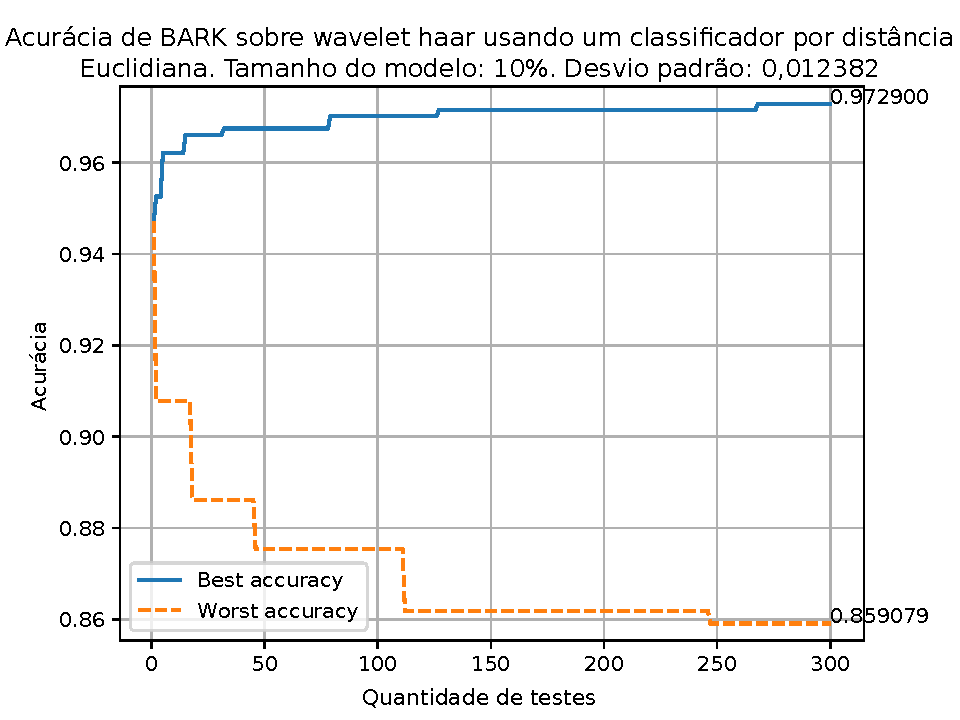
\includegraphics[width=\linewidth]{../monography/images/results/confusionMatrices/classifier_Euclidian_10}
				\caption{Acurácia \textit{X} quantidade de testes - Distância Euclidiana, modelo a 10\%}
			\end{figure}
			
			\column{0.5\textwidth}
			\begin{figure}
				\centering
				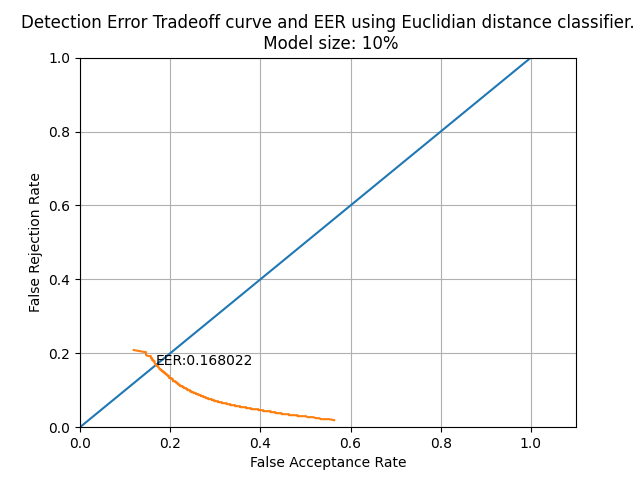
\includegraphics[width=\linewidth]{../monography/images/results/det/DET_for_classifier_Euclidian_10}
				\caption{Curva DET dos resultados de distância Euclidiana, modelo a 10\%}
			\end{figure}
		\end{columns}
	}
	\only<2>{
		\begin{columns}
			\column{0.5\textwidth}
			\begin{figure}
				\centering
				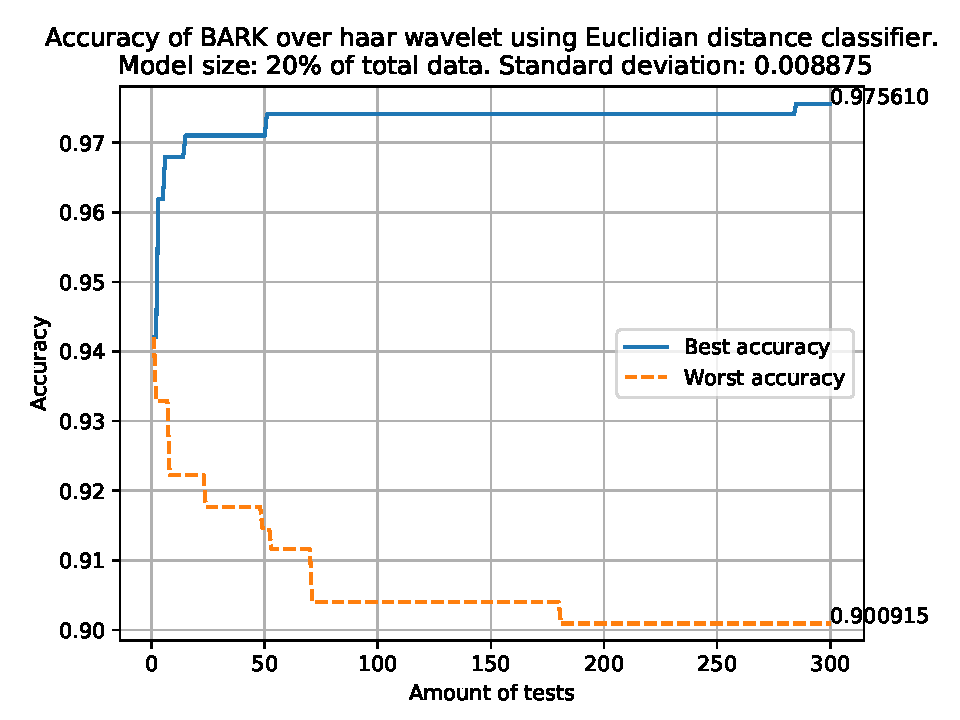
\includegraphics[width=\linewidth]{../monography/images/results/confusionMatrices/classifier_Euclidian_20}
				\caption{Acurácia \textit{X} quantidade de testes - Distância Euclidiana, modelo a 20\%}
			\end{figure}
			
			\column{0.5\textwidth}
			\begin{figure}
				\centering
				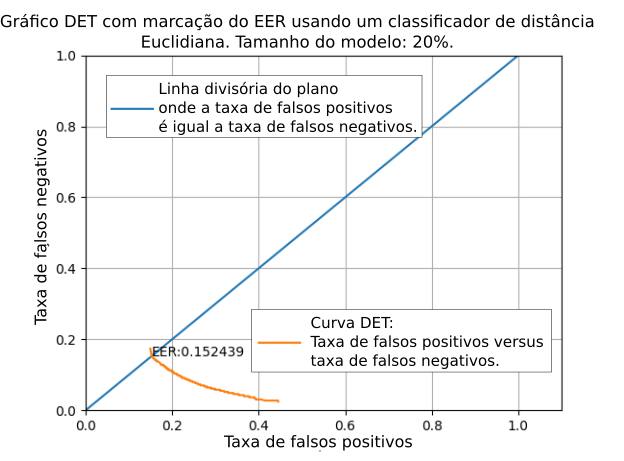
\includegraphics[width=\linewidth]{../monography/images/results/det/DET_for_classifier_Euclidian_20}
				\caption{Curva DET dos resultados de distância Euclidiana, modelo a 20\%}
			\end{figure}
		\end{columns}
	}
	\only<3>{
		\begin{columns}
			\column{0.5\textwidth}
			\begin{figure}
				\centering
				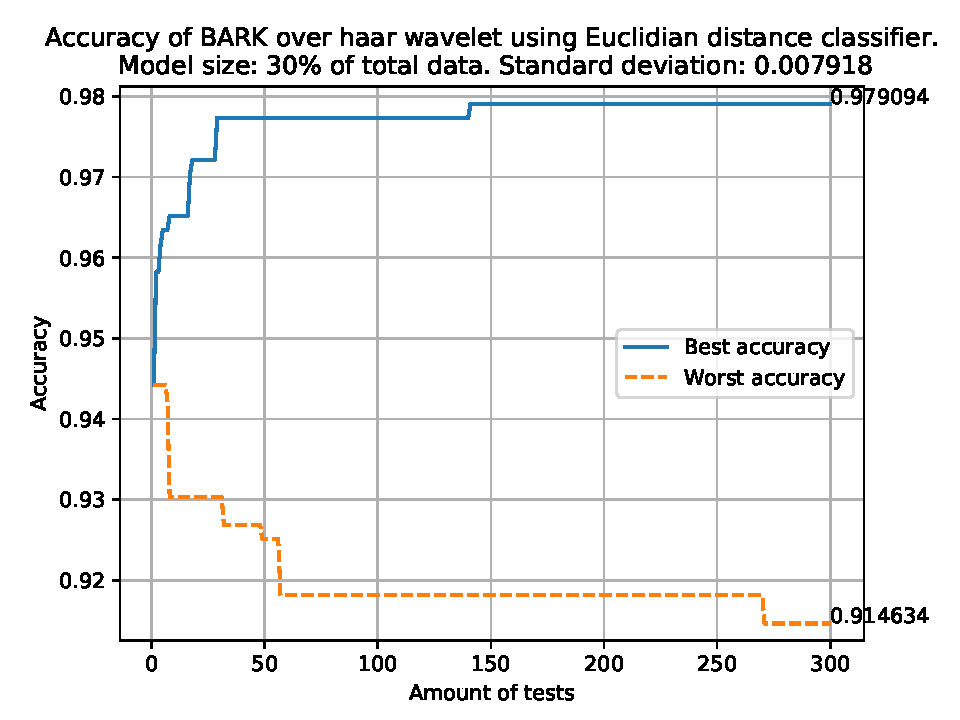
\includegraphics[width=\linewidth]{../monography/images/results/confusionMatrices/classifier_Euclidian_30}
				\caption{Acurácia \textit{X} quantidade de testes - Distância Euclidiana, modelo a 30\%}
			\end{figure}
			
			\column{0.5\textwidth}
			\begin{figure}
				\centering
				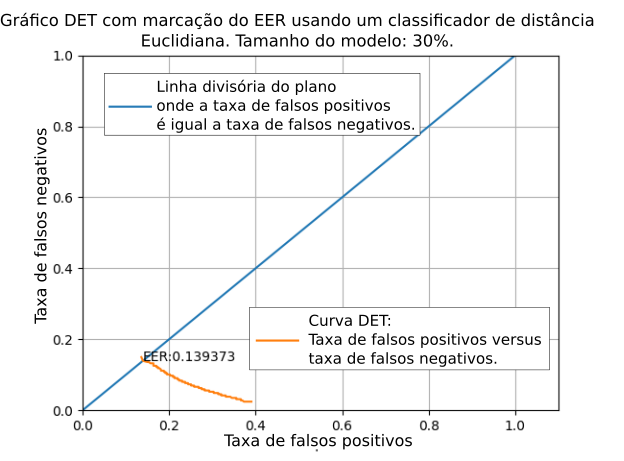
\includegraphics[width=\linewidth]{../monography/images/results/det/DET_for_classifier_Euclidian_30}
				\caption{Curva DET dos resultados de distância Euclidiana, modelo a 30\%}
			\end{figure}
		\end{columns}
	}
	\only<4>{
		\begin{columns}
			\column{0.5\textwidth}
			\begin{figure}
				\centering
				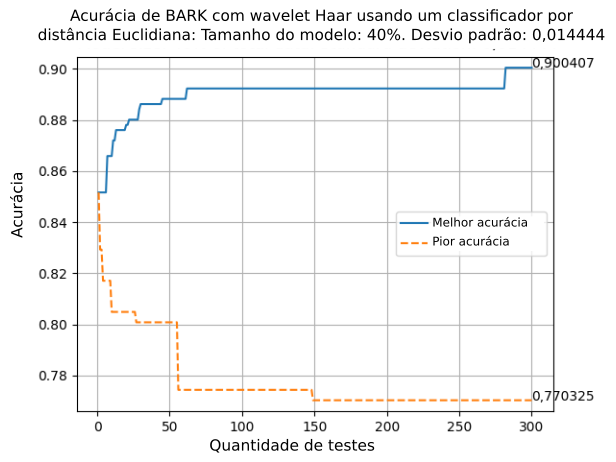
\includegraphics[width=\linewidth]{../monography/images/results/confusionMatrices/classifier_Euclidian_40}
				\caption{Acurácia \textit{X} quantidade de testes - Distância Euclidiana, modelo a 40\%}
			\end{figure}
			
			\column{0.5\textwidth}
			\begin{figure}
				\centering
				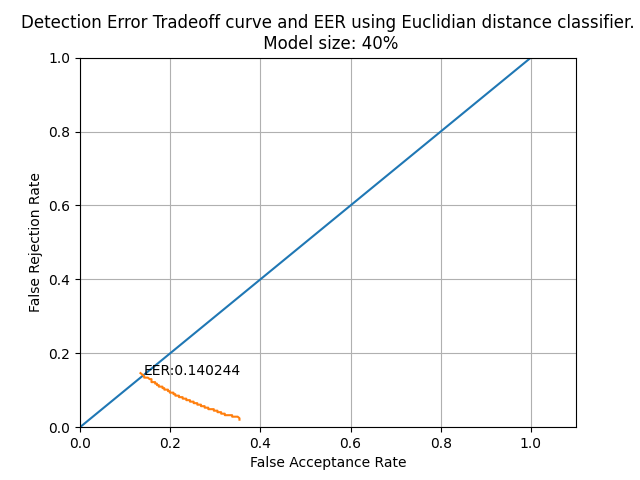
\includegraphics[width=\linewidth]{../monography/images/results/det/DET_for_classifier_Euclidian_40}
				\caption{Curva DET dos resultados de distância Euclidiana, modelo a 40\%}
			\end{figure}
		\end{columns}
	}
	\only<5>{
		\begin{columns}
			\column{0.5\textwidth}
			\begin{figure}
				\centering
				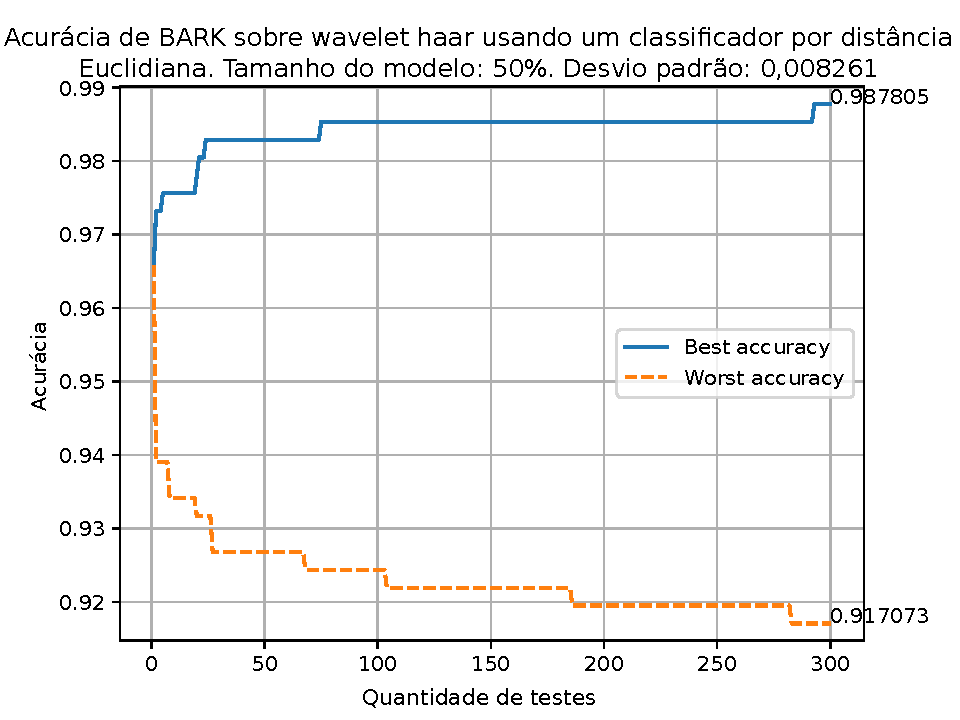
\includegraphics[width=\linewidth]{../monography/images/results/confusionMatrices/classifier_Euclidian_50}
				\caption{Acurácia \textit{X} quantidade de testes - Distância Euclidiana, modelo a 50\%}
			\end{figure}
			
			\column{0.5\textwidth}
			\begin{figure}
				\centering
				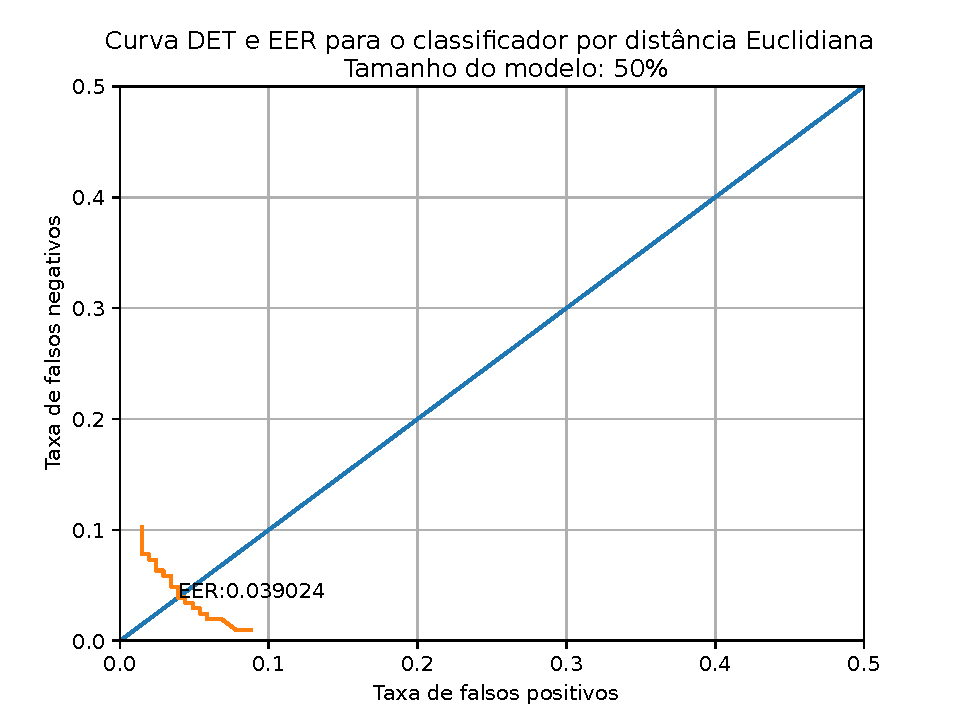
\includegraphics[width=\linewidth]{../monography/images/results/det/DET_for_classifier_Euclidian_50}
				\caption{Curva DET dos resultados de distância Euclidiana, modelo a 50\%}
			\end{figure}
		\end{columns}
	}
\end{frame}

\begin{frame}
	\frametitle{Procedimento 02}
	\framesubtitle{Acurácias e EER para distância Manhattan}
	\only<1>{
		\begin{columns}
			\column{0.5\textwidth}
			\begin{figure}
				\centering
				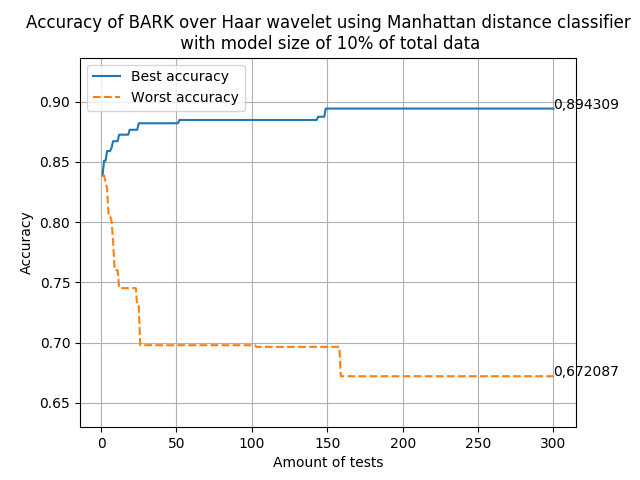
\includegraphics[width=\linewidth]{../monography/images/results/confusionMatrices/classifier_Manhattan_10.png}
				\caption{Acurácia \textit{X} quantidade de testes - Distância Manhattan, modelo a 10\%}
			\end{figure}
			
			\column{0.5\textwidth}
			\begin{figure}
				\centering
				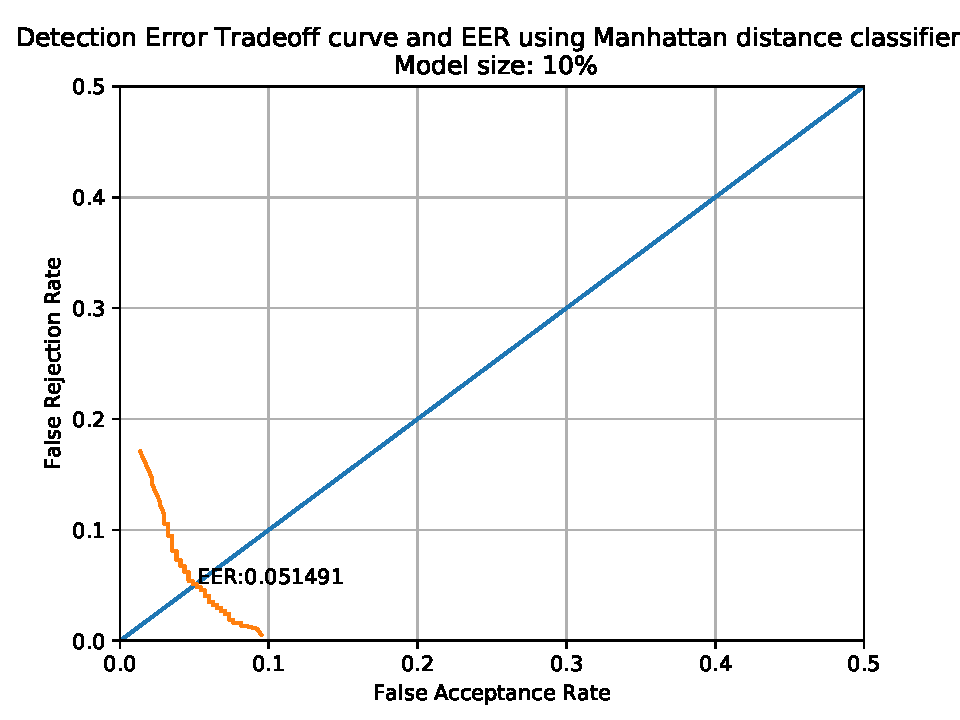
\includegraphics[width=\linewidth]{../monography/images/results/det/DET_for_classifier_Manhattan_10}
				\caption{Curva DET dos resultados de distância Manhattan, modelo a 10\%}
			\end{figure}
		\end{columns}
	}
	\only<2>{
		\begin{columns}
			\column{0.5\textwidth}
			\begin{figure}
				\centering
				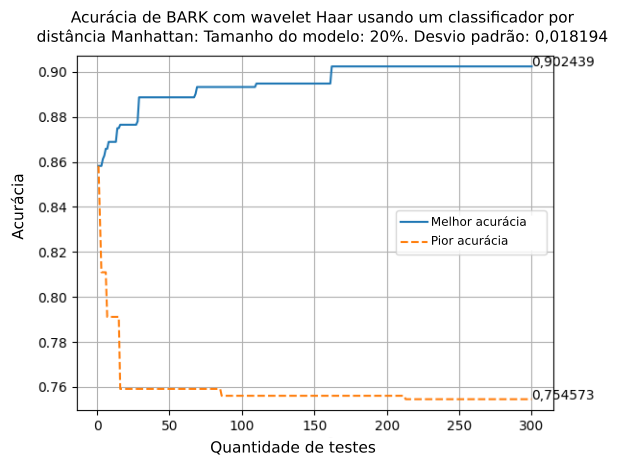
\includegraphics[width=\linewidth]{../monography/images/results/confusionMatrices/classifier_Manhattan_20.png}
				\caption{Acurácia \textit{X} quantidade de testes - Distância Manhattan, modelo a 20\%}
			\end{figure}
			
			\column{0.5\textwidth}
			\begin{figure}
				\centering
				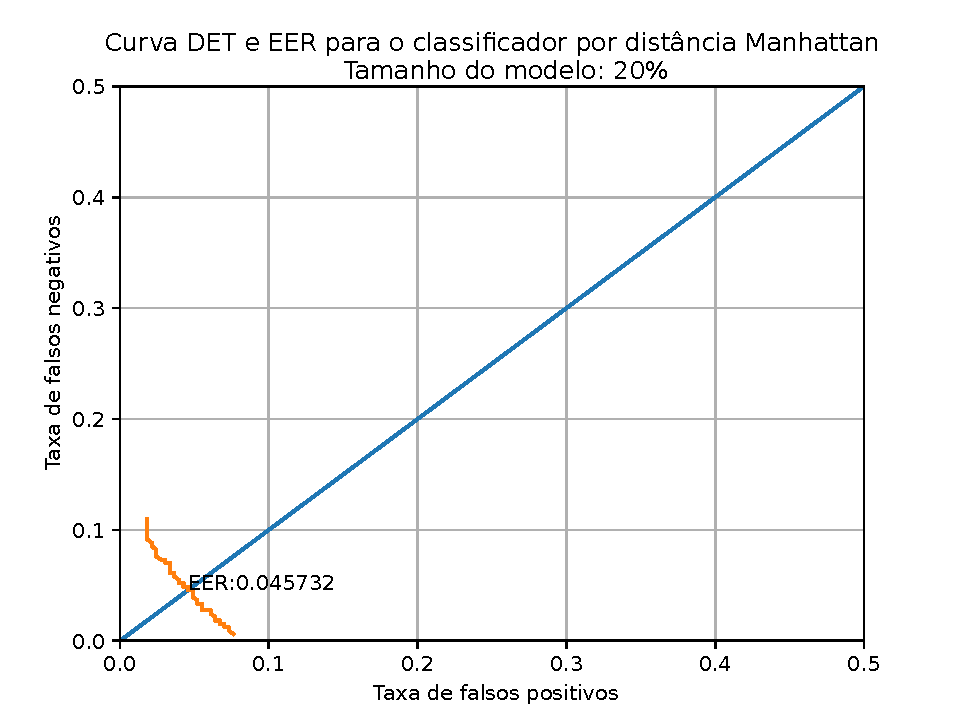
\includegraphics[width=\linewidth]{../monography/images/results/det/DET_for_classifier_Manhattan_20}
				\caption{Curva DET dos resultados de distância Manhattan, modelo a 20\%}
			\end{figure}
		\end{columns}
	}
	\only<3>{
		\begin{columns}
			\column{0.5\textwidth}
			\begin{figure}
				\centering
				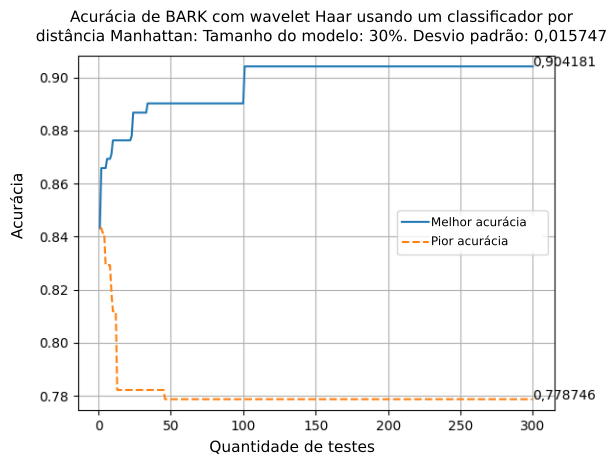
\includegraphics[width=\linewidth]{../monography/images/results/confusionMatrices/classifier_Manhattan_30.png}
				\caption{Acurácia \textit{X} quantidade de testes - Distância Manhattan, modelo a 30\%}
			\end{figure}
			
			\column{0.5\textwidth}
			\begin{figure}
				\centering
				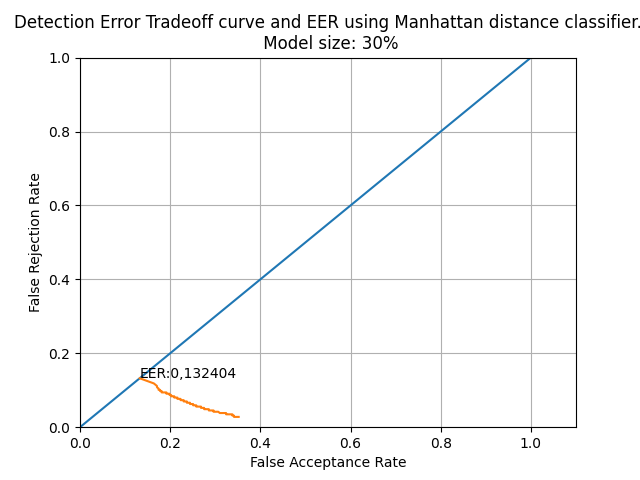
\includegraphics[width=\linewidth]{../monography/images/results/det/DET_for_classifier_Manhattan_30}
				\caption{Curva DET dos resultados de distância Manhattan, modelo a 30\%}
			\end{figure}
		\end{columns}
	}
	\only<4>{
		\begin{columns}
			\column{0.5\textwidth}
			\begin{figure}
				\centering
				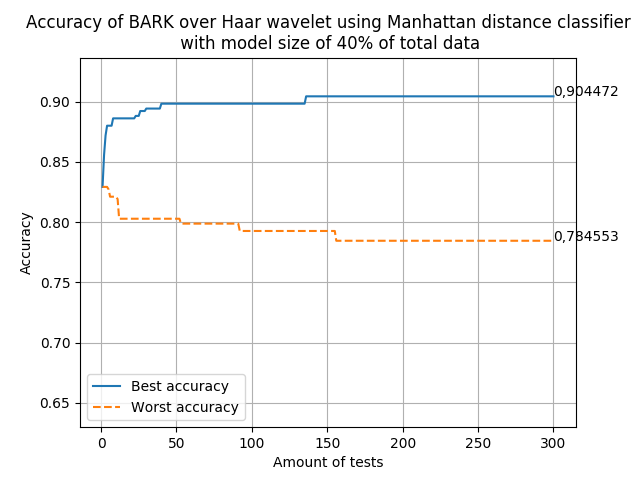
\includegraphics[width=\linewidth]{../monography/images/results/confusionMatrices/classifier_Manhattan_40.png}
				\caption{Acurácia \textit{X} quantidade de testes - Distância Manhattan, modelo a 40\%}
			\end{figure}
			
			\column{0.5\textwidth}
			\begin{figure}
				\centering
				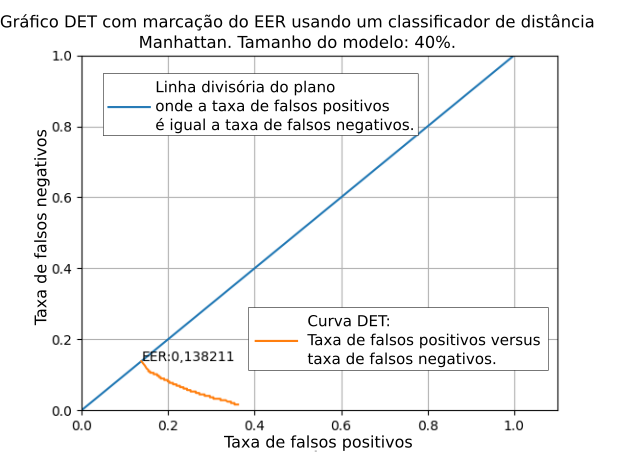
\includegraphics[width=\linewidth]{../monography/images/results/det/DET_for_classifier_Manhattan_40}
				\caption{Curva DET dos resultados de distância Manhattan, modelo a 40\%}
			\end{figure}
		\end{columns}
	}
	\only<5>{
		\begin{columns}
			\column{0.5\textwidth}
			\begin{figure}
				\centering
				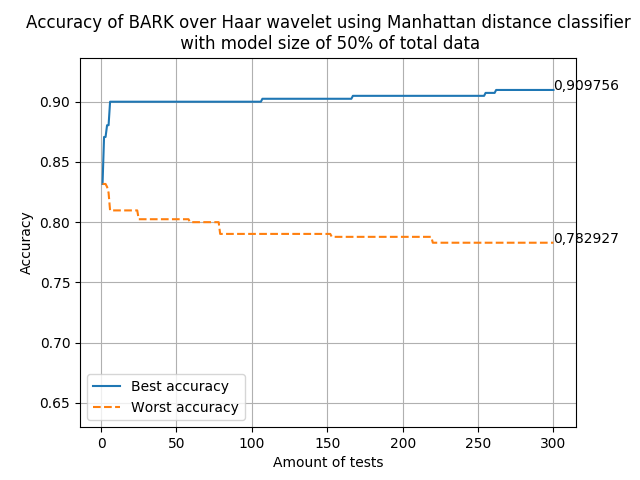
\includegraphics[width=\linewidth]{../monography/images/results/confusionMatrices/classifier_Manhattan_50.png}
				\caption{Acurácia \textit{X} quantidade de testes - Distância Manhattan, modelo a 50\%}
			\end{figure}
			
			\column{0.5\textwidth}
			\begin{figure}
				\centering
				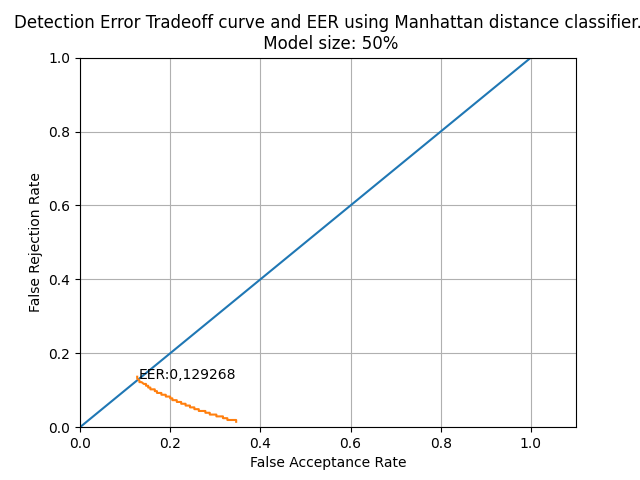
\includegraphics[width=\linewidth]{../monography/images/results/det/DET_for_classifier_Manhattan_50}
				\caption{Curva DET dos resultados de distância Manhattan, modelo a 50\%}
			\end{figure}
		\end{columns}
	}
\end{frame}

\begin{frame}
	\frametitle{Procedimento 02}
		\framesubtitle{Síntese}
		\par Dentre os testes realizados o melhores resultados foram:
		\begin{itemize}
			\item Distância Euclidiana $\rightarrow$ Acurácia: 0,904878 - ERR: 0,136585.
			\item Distância Manhattan $\rightarrow$ Acurácia: 0,909756 - ERR: 0,129268.
		\end{itemize}
\end{frame}
		\begin{frame}
	\frametitle{Procedimento 03}
	\begin{itemize}
		\item 
	\end{itemize}
\end{frame}
		\begin{frame}
	\frametitle{Testes Complementares}
	\begin{itemize}
		\item 
	\end{itemize}
\end{frame}	
		
	\section{Conclusões e Trabalhos Futuros}
		\begin{frame}
	\frametitle{Conclusões e Trabalhos Futuros}
	
	\only<1>{
		\framesubtitle{Conclusões}
		\begin{itemize}
			\item A engenharia paraconsistente de características foi de grande ajuda.
			\item O tipo de \textit{wavelet} utilizada na decomposição dos sinais influencia na criação dos vetores de características.
			\item A combinação \textit{wavelet-packet Haar + escala Bark} foi a melhor.
			\item A combinação \textit{wavelet-packet daubechies 54 + escala Mel} foi a pior.
			\item A escala \textit{Bark} é superior a \textit{MEL} por promover um espalhamento horizontal maior dos valores para os vetores de características.
		\end{itemize}
	}

	\only<2>{
		\framesubtitle{Trabalhos futuros}
		\begin{itemize}
			\item Explorar os resultados das transformadas \textit{wavelets} até um certo nível somente, em oposição a transformações sucessivas.
			\item Separar os componentes de alta e baixa frequência do sinal aparenta ser uma boa base para verificação de \textit{voice spoofing} devido a natureza ruidosa do sinal deste ataque.
			\item Focar a análise em bandas de frequência superiores.
		\end{itemize}
	}
\end{frame}
	
	\begin{frame}[allowframebreaks]
		\frametitle{Referências}
		\bibliography{bibliography.bib}
	\end{frame}
	
\end{document}